% =====================================================================
%  Generative AI -- Internal Assessment report
%  Solver-Verified Text-Conditioned Sokoban Level Generation
%
%  Build:  pdflatex report.tex   (three passes, for the ToC)
%  Every number in this document is read from a committed artifact under
%  ../results/.  Nothing is illustrative.
% =====================================================================
\documentclass[11pt,a4paper]{report}

\usepackage[T1]{fontenc}
\usepackage[utf8]{inputenc}
\usepackage{mathptmx}
\usepackage[scaled=0.90]{helvet}
\usepackage{courier}
\usepackage{amsmath,amssymb}
\usepackage[a4paper,left=2.3cm,right=2.2cm,top=2.2cm,bottom=2.3cm]{geometry}
\usepackage{graphicx}
\usepackage{booktabs}
\usepackage{array}
\usepackage{tabularx}
\usepackage{longtable}
\usepackage{multirow}
\usepackage{xcolor}
\usepackage{titlesec}
\usepackage[font=small,labelfont=bf,skip=6pt]{caption}
\usepackage{enumitem}
\usepackage{fancyhdr}
\usepackage{float}
\usepackage{microtype}
\usepackage[hidelinks,bookmarks=true]{hyperref}

\definecolor{accent}{HTML}{2F5C96}
\definecolor{accentlight}{HTML}{E8EEF6}
\definecolor{warm}{HTML}{B4652F}
\definecolor{rulegrey}{HTML}{9A9AA6}
\definecolor{softgrey}{HTML}{F4F4F7}

\hypersetup{linkcolor=accent, citecolor=accent, urlcolor=accent,
            colorlinks=false}

% === headings =======================================================
\titleformat{\chapter}[display]
  {\normalfont\sffamily\bfseries\color{accent}}
  {\filright\normalsize\sffamily\color{rulegrey}CHAPTER \thechapter}
  {4pt}
  {\Large\raggedright}
  [\vspace{2pt}{\color{accent}\titlerule[1.1pt]}]
\titlespacing*{\chapter}{0pt}{-16pt}{22pt}

\titleformat{\section}
  {\normalfont\sffamily\large\bfseries\color{accent}}{\thesection}{0.7em}{}
\titleformat{\subsection}
  {\normalfont\sffamily\normalsize\bfseries}{\thesubsection}{0.6em}{}
\titlespacing*{\section}{0pt}{14pt}{5pt}
\titlespacing*{\subsection}{0pt}{10pt}{3pt}

\pagestyle{fancy}
\fancyhf{}
\renewcommand{\headrulewidth}{0.4pt}
\fancyhead[L]{\footnotesize\sffamily\color{rulegrey}Solver-Verified Sokoban
              Level Generation}
\fancyhead[R]{\footnotesize\sffamily\color{rulegrey}\thepage}
\fancypagestyle{plain}{\fancyhf{}\renewcommand{\headrulewidth}{0pt}
                       \fancyfoot[C]{\footnotesize\sffamily\color{rulegrey}\thepage}}

\setlength{\parskip}{3.5pt}
\setlength{\parindent}{0pt}
\setlength{\emergencystretch}{2em}
\renewcommand{\arraystretch}{1.14}

% Thirteen figures and twelve tables in a single-column report: the default
% float parameters defer them so aggressively that pages end up two-thirds
% empty.  Allowing more float area per page packs each one next to the text
% that refers to it.
\renewcommand{\topfraction}{0.92}
\renewcommand{\bottomfraction}{0.70}
\renewcommand{\textfraction}{0.07}
\renewcommand{\floatpagefraction}{0.78}
\setcounter{topnumber}{3}
\setcounter{bottomnumber}{2}
\setcounter{totalnumber}{4}
\setlength{\textfloatsep}{12pt plus 3pt minus 3pt}
\setlength{\intextsep}{11pt plus 3pt minus 3pt}

\newcommand{\keyfinding}[1]{%
  \par\vspace{5pt}%
  \noindent\fcolorbox{accent}{accentlight}{%
    \begin{minipage}{\dimexpr\linewidth-2\fboxsep-2\fboxrule\relax}
      \small #1
    \end{minipage}}%
  \par\vspace{6pt}}

\newcommand{\tile}[1]{\texttt{#1}}

\begin{document}

% =====================================================================
% TITLE PAGE
% =====================================================================
\begin{titlepage}
\centering
\vspace*{0.4cm}

{\sffamily\large\bfseries K.\,J.\ SOMAIYA SCHOOL OF ENGINEERING}\\[3pt]
{\sffamily\normalsize Somaiya Vidyavihar University, Mumbai}\\[4pt]
{\sffamily\small Department of Artificial Intelligence \& Data Science}\\[18pt]

{\color{accent}\rule{\textwidth}{1.2pt}}\\[16pt]

{\sffamily\small\color{rulegrey} INTERNAL ASSESSMENT: GENERATIVE ARTIFICIAL
INTELLIGENCE}\\[20pt]

{\sffamily\LARGE\bfseries Solver-Verified Text-Conditioned\\[6pt]
Sokoban Level Generation}\\[14pt]

{\sffamily\large\itshape Autoregressive Models Can Count,\\ One-Shot Decoders
Cannot}\\[16pt]

{\color{accent}\rule{\textwidth}{1.2pt}}\\[22pt]

\begin{minipage}{0.86\textwidth}
\centering\small
A comparison of three generative model families (a decoder-only
transformer, a conditional variational autoencoder and a conditional
generative adversarial network) on the task of generating playable
$10\times10$ Sokoban puzzles from short text captions, evaluated with an
\textbf{exhaustive A* solver} used as a decision procedure rather than with a
learned or heuristic proxy metric.
\end{minipage}

\vspace{26pt}

{\sffamily\normalsize\bfseries Submitted by}\\[10pt]

\begin{tabular}{@{}l c l@{}}
\toprule
\textbf{Name} & \textbf{Roll Number} & \textbf{Class} \\
\midrule
Aayush Kumar Tiwari & 16014223003 & LY AI \& DS B \\
Prateeksha Kini     & 16014223061 & LY AI \& DS B \\
\bottomrule
\end{tabular}

\vfill

{\small\sffamily Academic Year 2025--26}\\[4pt]
{\footnotesize\sffamily\color{rulegrey}
All code, checkpoints, generated levels and result artifacts accompany this
report.\\
Every numeric claim below is traceable to a committed JSON artifact.}

\end{titlepage}

% =====================================================================
% ABSTRACT
% =====================================================================
\pagenumbering{roman}
\setcounter{page}{2}

\chapter*{Abstract}
\addcontentsline{toc}{chapter}{Abstract}
\markboth{Abstract}{Abstract}

Generative models are almost always judged by proxies. Perplexity does not tell
you whether a program runs, and a discriminator score does not tell you whether
a game level can be finished. This project asks what changes when the proxy is
removed entirely.

We generate $10\times10$ Sokoban puzzles from short natural-language captions
such as \texttt{"hard, \textasciitilde 40 moves, dense walls, corridors, boxes
scattered"}, and we check every single generated level with an
\textbf{exhaustive A* solver}. Because the state space of a $10\times10$ level
with four boxes is finite and every pruning rule we use is sound, running the
search to exhaustion is a \emph{proof} that no solution exists. The verifier is
therefore a decision procedure, not a one-sided test, and we report three
outcomes (\emph{solved}, \emph{proven unsolvable}, \emph{timed out}) and
never collapse them into two.

Three generative families are compared at roughly comparable scale: a
$10.7$M-parameter decoder-only transformer written from scratch, a
$1.1$M-parameter conditional VAE, and a $1.1$M-parameter conditional GAN, plus
a DistilGPT-2 pretraining ablation. The central finding is architectural. A
valid level needs \emph{exactly} one player, four boxes and four goals. A
transformer that emits the grid cell by cell can count what it has already
placed and reaches $82.6\%$ structural validity with no help; a VAE that
decodes all $100$ cells at once from a single latent vector cannot, and produces
\textbf{zero} valid levels in $100{,}000$ draws under argmax decoding. Applying
a hard constraint to the logits during sampling closes that gap deterministically
at $100\%$ validity.

Three further results complicate the simple story. Solvability does not follow
from validity: an empty room with no interior walls is already solvable
$23.4\%$ of the time against the transformer's $49.6\%$. Repairing the VAE's
counting errors gives $76.6\%$ solvability, \emph{above} the transformer,
which locates the autoregressive advantage in counting rather than in spatial
understanding. And measuring across three training seeds proved essential:
solvability moves by $\pm 7.0$ points across seeds while validation loss moves
by $\pm 0.005$, so validation loss is a poor proxy for the property actually
being evaluated.

\vspace{6pt}
\textbf{Keywords:} procedural content generation, autoregressive models,
variational autoencoders, generative adversarial networks, constrained
decoding, verification, Sokoban.

\vspace{10pt}
\noindent\textit{Provenance.} This project is a replication and extension of
Todd et al.\ (FDG 2023), \emph{Level Generation Through Large Language Models}.
The data-scaling finding, the solvability-versus-conditioning setup and the
tokenization finding are theirs; we claim none of them. No novelty is claimed
anywhere in this report.

% =====================================================================
\tableofcontents
\listoffigures
\listoftables

\cleardoublepage
\pagenumbering{arabic}
\setcounter{page}{1}

% =====================================================================
\chapter{Introduction}

\section{Background and motivation}

A generative model is only as trustworthy as the thing that scores it. In text
generation we use perplexity; in image generation, FID; in procedural content
generation, hand-designed heuristics or a learned discriminator. All of these
share a weakness: they measure whether the output \emph{resembles} the training
data, not whether it \emph{works}.

Some domains do better. HumanEval runs unit tests on generated code, Lean checks
generated proofs, and text-to-SQL is scored by executing the query. So it is
simply not true that no metric can tell you whether a generated artifact
functions. But every one of those verifiers is \textbf{sound but incomplete}: a
passing unit test does not prove a program correct, and a failing test suite
cannot prove a program wrong; it can only fail to find a counter-example. The
verifier answers ``yes'' reliably and ``no'' only provisionally.

Sokoban is unusual because it admits the other kind of verifier. A
$10\times10$ grid with four boxes has a state space that is finite and small
enough to search exhaustively. Given pruning rules that are \emph{sound},
meaning they discard only states from which no solution could exist, draining
the search frontier to empty is a constructive proof that the level is
unsolvable. That makes the verifier a \textbf{decision procedure}, and it lets
us ask a question most generative-model evaluations cannot ask: not ``does this
look right?'' but ``is this actually playable, yes or no?''

\begin{figure}[!htb]
\centering
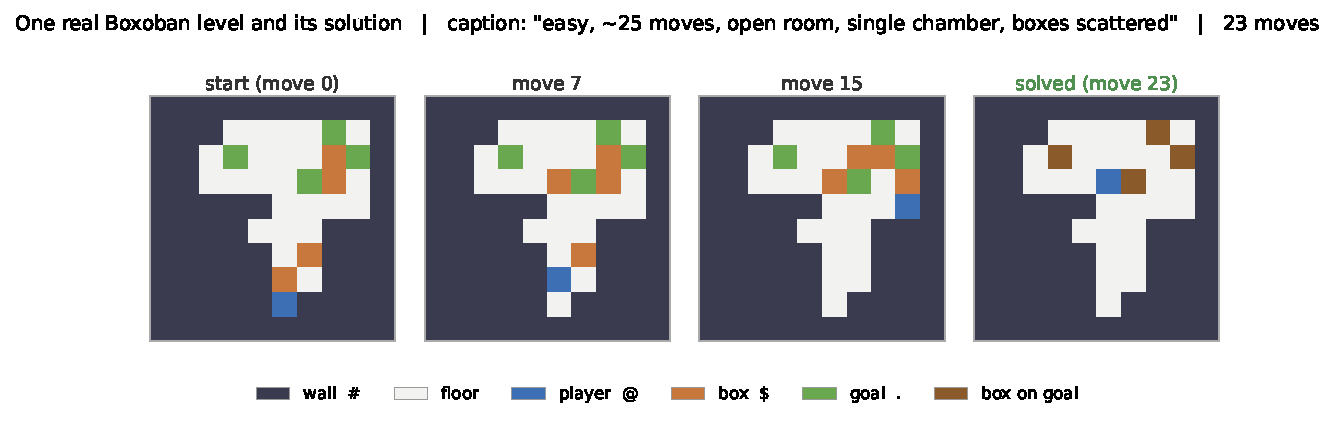
\includegraphics[width=\textwidth]{figures/r1_sokoban_basics.pdf}
\caption[What a Sokoban level is]{Sokoban in one picture. The player
(\textcolor{accent}{blue}) pushes boxes (\textcolor{warm}{orange}) onto goal
squares (green); boxes can only be \emph{pushed}, never pulled, so a box shoved
into a corner is lost forever. The level is solved when every box stands on a
goal. This is a real held-out Boxoban level, replayed under its published
$23$-move solution. The caption above it is the kind of text our models are
conditioned on, and it is computed from the grid, not hand-written.}
\label{fig:sokoban}
\end{figure}

\section{Problem statement}

Given a short natural-language caption describing a puzzle's difficulty,
solution length, wall density, corridor structure and box layout, generate a
$10\times10$ Sokoban level that is (i) \emph{structurally valid}, with exactly
one player, four boxes, four goals and a complete wall border, (ii)
\emph{solvable}, as proven by exhaustive search, (iii) \emph{novel}, not a copy
of a training level, and (iv) \emph{faithful to the caption}.

The four requirements pull against each other, and that is the point. Copying a
training level maximises solvability and destroys novelty. Generating an empty
room gives decent solvability and ignores the caption. A single headline number
hides all of this, so the results in this report are always presented as a joint
constraint over several axes rather than as one score.

\section{Objectives}

\begin{enumerate}[leftmargin=1.5em,itemsep=2pt]
\item Build and \emph{validate} an exhaustive A* Sokoban solver, and establish
      before anything else is measured that it can be trusted as ground truth.
\item Train three generative model families (autoregressive transformer,
      conditional VAE, conditional GAN) at roughly comparable parameter
      counts on the same data with the same conditioning information.
\item Test a specific architectural hypothesis: that autoregressive decoding can
      satisfy hard counting constraints that one-shot decoding cannot.
\item Implement constrained decoding (a hard logit mask) and grid repair, and
      report them as separate rows so that \emph{counting} and \emph{spatial
      understanding} are measured separately rather than merged.
\item Measure controllability per caption attribute, and quantify how far the
      results move when only the random seed changes.
\item Report negative results such as out-of-distribution failure, mode
      collapse and inverted rankings as findings rather than as problems to
      tune away.
\end{enumerate}

\section{Scope and non-goals}

This is an \emph{engineering and evaluation} project, not an architecture
proposal. We contribute no new model design. The models are deliberately
standard so that the comparison is about the decoding structure, not about
clever tricks. Concretely:

\begin{itemize}[leftmargin=1.5em,itemsep=1pt]
\item One game, one grid size: $10\times10$, four boxes, four goals. Nothing
      here shows the finding generalises to other tile games or grid sizes.
\item All training was done on a single laptop RTX 3050 with 6\,GB of VRAM. Model
      sizes are chosen to fit that budget honestly, not to be competitive with
      large models.
\item Hyperparameters were chosen once and never swept. They are reported as
      \emph{admitted defaults} throughout rather than justified after the fact.
\item No novelty is claimed. Similar pipelines exist in the literature and are
      cited in Chapter~\ref{ch:lit}.
\end{itemize}

\section{Organisation of this report}

Chapter~\ref{ch:lit} surveys related work and states precisely what is borrowed
and what is added. Chapter~\ref{ch:data} covers the dataset and a set of
data-quality findings that turned out to matter. Chapter~\ref{ch:models}
describes the three generative families and the constrained decoding scheme in
which the central hypothesis is tested. Chapter~\ref{ch:eval} describes the
solver and the evaluation protocol, and Chapter~\ref{ch:impl} the
implementation. Chapter~\ref{ch:results} presents the results and the failure
analysis, and Chapter~\ref{ch:conclusion} states the limitations and concludes.

% =====================================================================
\chapter{Literature Survey}
\label{ch:lit}

\section{Procedural content generation via machine learning}

Procedural content generation via machine learning (PCGML) has used
autoencoders and GANs over tile grids for years. The standard recipe is to
encode a level as a 2-D grid of tile categories, train a generative model over
that grid, and evaluate with a mixture of visual inspection, tile-distribution
statistics and an agent that tries to play the level. Our models are drawn from
exactly this tradition; the contribution is not the architecture but the
verifier attached to it.

\section{Language models for level generation}

Todd et al.\ (FDG 2023) fine-tune GPT-2 variants to generate Sokoban levels from
a character encoding and study how solvability scales with the amount of
training data and with the choice of tokenization. \textbf{This project is a
replication and extension of that work.} The data-scaling result, the
solvability-versus-conditioning setup and the tokenization finding are theirs,
and we claim none of them.

MarioGPT conditions level generation on natural language for \emph{Super Mario
Bros.}, checking playability with an A* agent. That agent is a sound but
incomplete verifier: it can confirm a level is playable but cannot prove that
one is not. The distinction matters for how results may be reported, and it is
the specific gap this project addresses.

\section{Verification versus proxy metrics}

The most relevant precedents come from outside PCG: HumanEval executes unit
tests against generated programs, interactive theorem provers check generated
proofs mechanically, and text-to-SQL benchmarks score by execution accuracy. In
every case the verifier is sound but incomplete. A decision procedure, which is what
an exhausted search over a finite state space gives us, is strictly stronger,
and is rarely available in generative evaluation.

\section{Sokoban and search}

Sokoban is PSPACE-complete in general, and the solver literature is built on
domain-specific pruning. Our solver is deliberately conservative and uses only
two prunes, both provably sound, because an \emph{unsound} prune produces false
proofs of unsolvability, the worst failure mode available here, since it
corrupts the headline number invisibly and in a flattering direction. The
Boxoban corpus we use was introduced for model-free planning research and
generated by reverse play from an already-solved state.

\section{What this project adds}

Relative to the work it replicates, three things are added:

\begin{enumerate}[leftmargin=1.5em,itemsep=2pt]
\item \textbf{Constrained decoding with feasibility forcing}, which makes
      structural validity deterministic rather than learned, and lets us
      separate ``can the model count?'' from ``does the model understand the
      puzzle?''
\item \textbf{Three-way solver reporting} that distinguishes proven
      unsolvability from timeout, which is only possible because the verifier is
      a decision procedure.
\item \textbf{A controlled multi-family comparison} at comparable parameter
      counts, including one-shot decoders and four non-learned baselines that
      bound how the headline number may be interpreted.
\end{enumerate}

\begin{table}[!htb]
\centering\small
\caption{Where this project sits relative to the closest prior work.}
\label{tab:lit}
\begin{tabularx}{\textwidth}{@{}l l X@{}}
\toprule
\textbf{Work} & \textbf{Verifier} & \textbf{Relation to this project} \\
\midrule
Todd et al.\ 2023 & A* agent (sound, incomplete) &
Directly replicated and extended. Data-scaling and tokenization findings are
theirs. \\
MarioGPT & A* agent (sound, incomplete) &
Same text-conditioning idea, different game; cannot prove unplayability. \\
PCGML (autoencoders, GANs) & tile statistics, human inspection &
Source of our VAE and GAN baselines. \\
\textbf{This project} & \textbf{exhaustive A* (decision procedure)} &
Adds constrained decoding, three-way verdicts, and a controlled multi-family
comparison. \\
\bottomrule
\end{tabularx}
\end{table}

% =====================================================================
\chapter{Dataset and Caption Construction}
\label{ch:data}

\section{The Boxoban corpus}

We use the Boxoban \texttt{unfiltered} split: $100{,}000$ training levels,
$5{,}000$ from the \emph{official} validation split (we deliberately do not
carve a validation set out of train), and the $1{,}000$-level test split held
frozen for solver validation and used as the ``real levels'' ceiling row in
every results table. Solution lengths come from a published A* solution set.

\section{Verifying the format instead of assuming it}

Every property the representation depends on was verified rather than assumed.
The checks are cheap and each of them would have broken something silently had
it failed.

\begin{table}[!htb]
\centering\small
\caption[Verified dataset format properties]{Format properties verified before any modelling
(\texttt{results/data\_verification.json}).}
\label{tab:dataverify}
\begin{tabularx}{\textwidth}{@{}l X@{}}
\toprule
\textbf{Property} & \textbf{Finding} \\
\midrule
Tile alphabet & Exactly $\{$\tile{\#}, \tile{@}, \tile{\$}, \tile{.},
space$\}$ over $50$ level files. \textbf{Neither \tile{*} (box on goal) nor
\tile{+} (player on goal) occurs anywhere}, so a box never \emph{starts} on a
goal. \\
Grid invariants & $10{,}000$ of $10{,}000$ levels are $10\times10$ with a
complete wall border and exactly one player, four boxes and four goals. Zero
violations. \\
Line endings & Files are CRLF; the parser normalises them. \\
Solution units & \texttt{Steps} counts \textbf{player moves, not pushes}:
\texttt{Steps == len(Actions)} on $989/989$ well-formed rows, with digits
$0$--$3$ meaning Up, Right, Down, Left. \\
Floor components & Every Boxoban level has \textbf{exactly one} connected floor
region, measured over $20{,}000$ levels. \\
Cross-split leakage & Zero collisions between train and either held-out split.
\\
\bottomrule
\end{tabularx}
\end{table}

Two of these findings changed design decisions. The absence of \tile{*} and
\tile{+} is what makes the five-channel one-hot tensor, the six-symbol grid
vocabulary and the ``exactly four \tile{\$} and four \tile{.}'' constraint all
well-defined at once. And the floor-component result killed a planned caption
feature: ``number of connected floor regions'' is a \emph{constant} on this
corpus, so it carries no information and cannot bin anything. We replaced it with
mean floor degree, the average number of non-wall neighbours per floor cell,
which ranges from $2.19$ to $3.36$ and does discriminate.

\section{A data-quality finding: some published solutions are wrong}

The solution set documents rows whose action field is
\texttt{SEARCH\_STATE\_FAILED} or \texttt{NOT\_FOUND}. Beyond those, we found
rows that \emph{look} perfectly well-formed, a plain digit string, but
that \textbf{do not replay to a solved state}: $63$ of $1000$ ($6.3\%$) in the
test split and approximately $0.7\%$ in train. They fail by walking into a wall
or making an impossible push part-way through, and treating blocked moves as
no-ops rescues none of them; no direction convention or transposition rescues
them either.

\keyfinding{\textbf{Every solution used in this project is replay-validated
against an independent simulator, and levels whose solution does not replay are
dropped}: $734$ of $100{,}000$ training levels ($0.73\%$), $373$ of $5{,}000$
validation levels and $74$ of $1{,}000$ test levels ($7.4\%$). A caption built
on a wrong solution length is worse than no example at all, because it teaches
the model a false association with full confidence.}

\section{Caption construction}

Five features are computed from each grid; \textbf{nothing is hand-labelled}.
The thresholds are the terciles and medians of the training distribution, so the
bins are balanced by construction.

\begin{table}[!htb]
\centering\small
\caption[The five caption features]{The five caption features and their measured bin boundaries
(\texttt{results/dataset\_build.json}).}
\label{tab:captions}
\begin{tabularx}{\textwidth}{@{}l X l@{}}
\toprule
\textbf{Feature} & \textbf{How it is computed} & \textbf{Boundary} \\
\midrule
Difficulty & solution length, binned by training terciles &
$\leq 26$ / $\leq 35$ / $> 35$ moves \\
Solution length & rounded to the nearest five moves & range $4$--$130$ \\
Wall density & interior \tile{\#} count $/\,64$, split at the training median &
$0.500$ \\
Connectivity & mean non-wall neighbours per floor cell, split at the median &
$2.889$ \\
Box clustering & mean pairwise Manhattan distance between boxes, split at the
median & $3.500$ \\
\bottomrule
\end{tabularx}
\end{table}

A caption reads, for example:

\begin{center}
\colorbox{softgrey}{\parbox{0.82\textwidth}{\centering\ttfamily\small
hard, \textasciitilde 40 moves, dense walls, corridors, boxes scattered}}
\end{center}

The same five features are encoded twice: as \textbf{caption text} for the
transformer and as a \textbf{$10$-dimensional vector} for the VAE and GAN. These
are different information channels, so the family comparison is not perfectly
controlled on conditioning. We state this rather than claim otherwise; it is
listed again in Chapter~\ref{ch:conclusion} as a limitation.

\section{Final splits and representations}

After replay validation, $99{,}266$ training rows, $4{,}627$ validation rows and
$926$ test rows survive. Each row carries the raw grid, the caption text, the
$10$-dimensional caption vector, and the verified solution length.

Two representations are derived from each grid:

\begin{itemize}[leftmargin=1.5em,itemsep=1pt]
\item \textbf{Character sequence} ($110$ characters: ten rows of ten tiles plus
      ten newlines) for the autoregressive models, wrapped as
      \texttt{<bos>}\,caption\,\texttt{<sep>}\,grid\,\texttt{<eos>}. Vocabulary
      is $48$ hand-written characters; the longest sequence observed is $176$
      tokens.
\item \textbf{Five-channel one-hot tensor} of shape $5\times10\times10$ for the
      one-shot decoders, one channel per tile type.
\end{itemize}

% =====================================================================
\chapter{Generative Models and Constrained Decoding}
\label{ch:models}

\section{Task formulation}

Let $c$ be a caption and $g$ a level. All four models estimate $p(g \mid c)$;
they differ entirely in \emph{how they factorise it}, and that factorisation is
the whole experiment.

\begin{align}
\textbf{Autoregressive:}\quad & p(g \mid c) = \prod_{t=1}^{110}
   p(g_t \mid g_{<t},\, c) \label{eq:ar}\\[2pt]
\textbf{One-shot latent:}\quad & p(g \mid c) = \int p(z \mid c)
   \prod_{i=1}^{100} p(g_i \mid z,\, c)\; dz \label{eq:oneshot}
\end{align}

Read the two products carefully, because the central hypothesis of this project
is visible in them. In Equation~\ref{eq:ar} the distribution over cell $t$ is
conditioned on \emph{every cell already emitted}, so the model can in principle
know how many boxes it has placed. In Equation~\ref{eq:oneshot} the cells are
conditionally independent given $z$: once the latent is drawn, no cell knows
what any other cell decided.

A valid Sokoban level requires \emph{exactly} one player, four boxes and four
goals. That is a constraint on the \emph{joint} distribution over cells. A
factorisation that makes cells conditionally independent can match the correct
\emph{marginal} rate of boxes without ever producing the correct \emph{number}
in any single sample.

\begin{figure}[!htb]
\centering
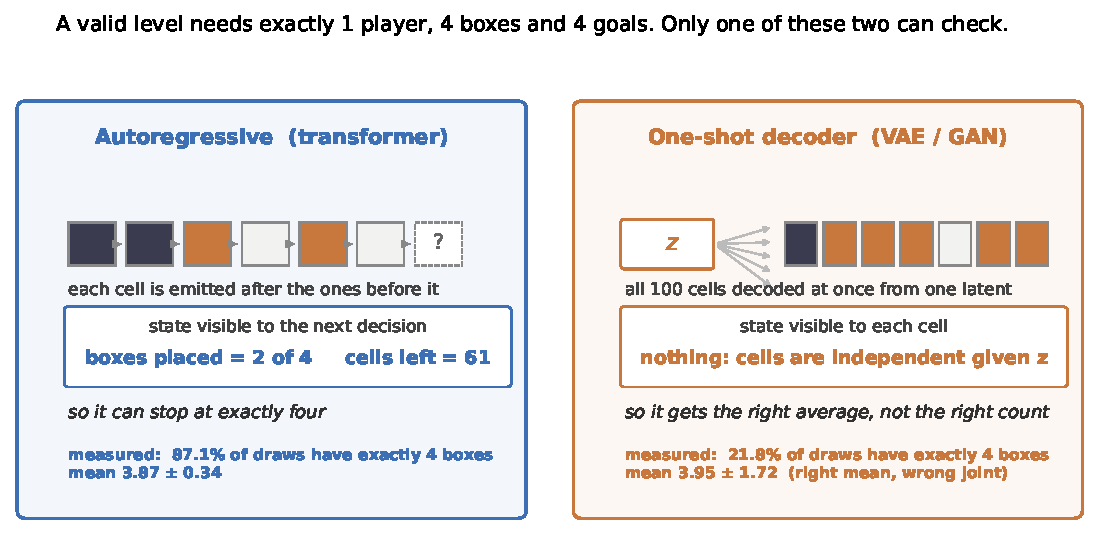
\includegraphics[width=\textwidth]{figures/r2_counting.pdf}
\caption[Why one-shot decoders cannot count]{The counting hypothesis, and the
measured outcome. An autoregressive decoder sees its own partial output, so it
can stop at four boxes; a one-shot decoder draws one latent and then decodes all
$100$ cells independently, so it has nothing to count with. The percentages are
measured over raw draws, valid or not.}
\label{fig:counting}
\end{figure}

\section{Transformer (primary system)}

A decoder-only transformer written from scratch: $d_{\text{model}} = 384$, $6$
layers, $6$ attention heads, $d_{\text{ff}} = 1536$, learned positional
embeddings, pre-norm residual blocks, GELU activations, dropout $0.1$, and tied
input/output embeddings, for a total of \textbf{$10{,}734{,}336$ parameters}.

We deliberately do \emph{not} use a fine-tuned pretrained model as the primary
system, so that the three-family comparison is roughly parameter-fair
($10.7$M against $1.1$M and $1.1$M) rather than pitting a stock $82$M
pretrained model against $1$M-parameter decoders. Pretraining is investigated
separately as an ablation in Section~\ref{sec:pretrain-model}.

The loss is next-token cross-entropy \textbf{masked over the caption prefix}, so
the model is trained to predict the grid given the caption, not to predict the
caption itself.

\section{Conditional variational autoencoder}

An MLP encoder and decoder over the $5\times10\times10$ one-hot tensor, latent
dimension $32$, hidden width $512$, for a total of
\textbf{$1{,}098{,}292$ parameters}.

Two design choices are worth stating because the obvious defaults are wrong here:

\begin{itemize}[leftmargin=1.5em,itemsep=2pt]
\item \textbf{Per-cell categorical cross-entropy, not MSE.} Mean squared error
      on a one-hot tile tensor treats the categorical channel axis as a metric
      space, as if ``wall'' were numerically halfway between ``floor'' and
      ``box''. It is a common and wrong default.
\item \textbf{Free bits rather than KL annealing} to prevent posterior collapse,
      with a floor of $0.05$ nats per latent dimension. It is one line of code
      with no schedule to tune. The measured KL was $8.8$ nats, far above the
      $1.6$-nat floor, so the posterior did not collapse.
\end{itemize}

MLPs rather than convolutions: a $10\times10$ grid does not factor cleanly for
strided convolutions, and at $100$ cells convolutions buy very little while
costing shape bugs.

\subsection{Two decoding protocols, both reported}

The VAE is reported under \textbf{two} decoding protocols, and both are
mandatory:

\begin{itemize}[leftmargin=1.5em,itemsep=2pt]
\item \textbf{Argmax:} take the most likely tile in each cell independently.
      This is the standard choice and it fails catastrophically, for a reason
      that is worth understanding: the argmax of a product of independent
      marginals is \emph{not} the mode of the joint distribution, and rare tiles
      are precisely what gets annihilated. Boxes occupy $4$ of $100$ cells;
      floor or wall wins almost everywhere.
\item \textbf{Per-cell sampling:} draw each cell from its own categorical
      distribution. This preserves the marginal tile rates and produces roughly
      the right \emph{number} of boxes in the wrong \emph{places}.
\end{itemize}

Reporting argmax alone would be an unfair protocol and would overstate the
conclusion, so both appear as separate rows in every table.

\section{Conditional generative adversarial network}

An MLP generator and discriminator, \textbf{$1{,}082{,}357$ parameters}
combined, using straight-through Gumbel-softmax discretisation with the
temperature annealed from $1.0$ to $0.3$, plus one-sided label smoothing at
$0.9$.

Discretisation is not optional here. Training on continuous logits and taking
the argmax only at sampling time is \emph{not} a valid option: the discriminator
can then separate real one-hot tensors from soft generator output purely by
per-cell entropy, training collapses onto that trivial discriminator, and the
generator learns nothing at all about layout.

This family was hard time-boxed at three hours. Mode collapse is reported as a
finding, not treated as a failure to be fixed.

\section{DistilGPT-2 ablation: does pretraining transfer?}
\label{sec:pretrain-model}

The ablation asks a specific question: does natural-language pretraining help in
a domain that shares \emph{no vocabulary} with the pretraining corpus?

To make the question sharp, the setup discards the $50257 \times 768$ token
embedding matrix and the tied language-model head, and re-initialises both for
our $48$-symbol vocabulary. Nothing lexical can transfer. Only the attention and
MLP blocks survive, leaving $43{,}352{,}064$ parameters.

\begin{figure}[!htb]
\centering
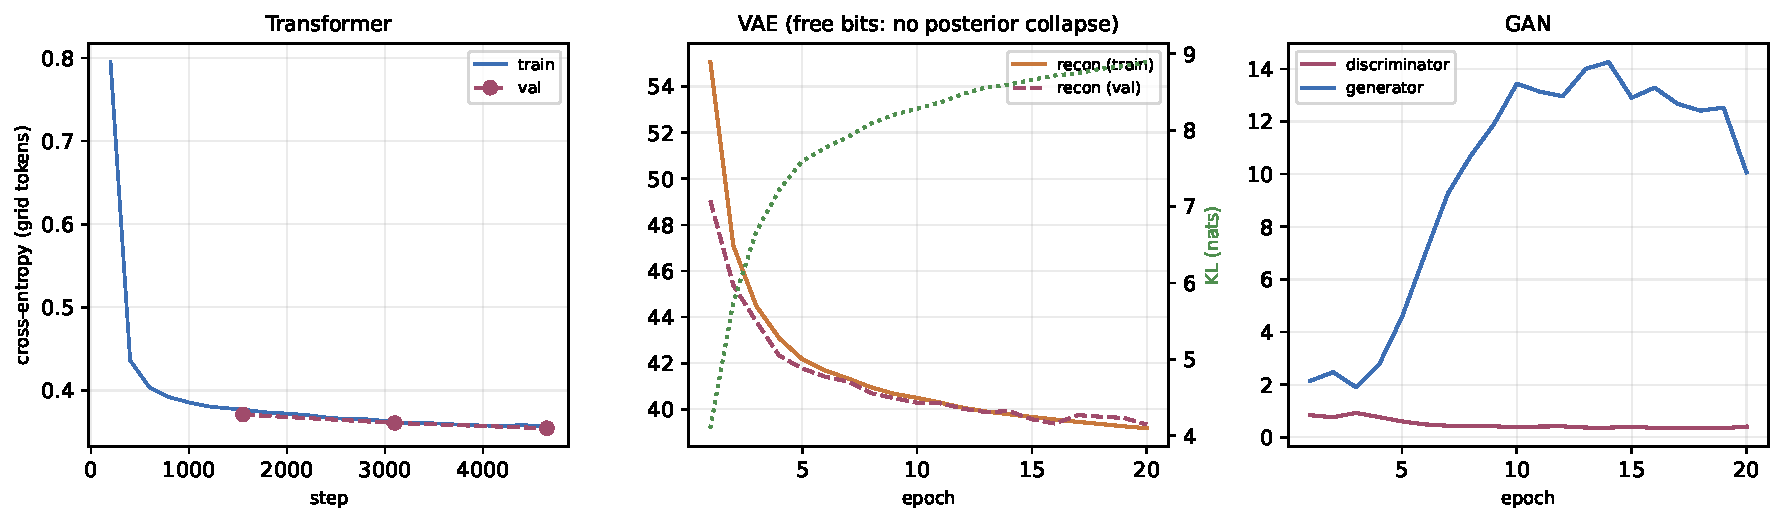
\includegraphics[width=\textwidth]{../figures/figB_training_curves.pdf}
\caption[Training curves for all three families]{Training behaviour of the three
families. \emph{Left:} the transformer converges smoothly with train and
validation loss tracking each other, so it is not overfitting. \emph{Centre:}
the VAE's reconstruction loss falls while the KL term rises to $8.8$ nats,
well above the $1.6$-nat free-bits floor, confirming the posterior did not
collapse. \emph{Right:} the GAN's generator loss climbs steadily while the
discriminator loss stays flat and low, which is the signature of a discriminator
that has won. This is mode collapse, and it is reported rather than tuned away.}
\label{fig:curves}
\end{figure}

\begin{table}[!htb]
\centering\small
\caption[The four models side by side]{The four models side by side. Parameter counts and training times are
read from \texttt{results/train\_*.json}; all runs used bf16 on one RTX 3050
(6\,GB).}
\label{tab:models}
\begin{tabularx}{\textwidth}{@{}l X X X X@{}}
\toprule
& \textbf{Transformer} & \textbf{Cond.\ VAE} & \textbf{Cond.\ GAN} &
  \textbf{DistilGPT-2} \\
\midrule
Architecture & decoder-only LM, from scratch & MLP encoder/decoder &
  MLP generator/discriminator & pretrained body, new vocabulary \\
Parameters & $10{,}734{,}336$ & $1{,}098{,}292$ & $1{,}082{,}357$ &
  $43{,}352{,}064$ \\
Conditioning & caption \textbf{text} prefix & caption \textbf{vector} (10-d) &
  caption \textbf{vector} (10-d) & caption \textbf{text} prefix \\
Output & $110$ characters, one at a time & $5\times10\times10$ logits, one shot &
  $5\times10\times10$ logits, one shot & $110$ characters, one at a time \\
Optimiser & AdamW, wd $0.01$ & Adam & Adam, $\beta=(0.5, 0.999)$ & AdamW \\
Learning rate & $3\mathrm{e}{-4}$\,\emph{(untuned)} &
  $1\mathrm{e}{-3}$\,\emph{(untuned)} & $2\mathrm{e}{-4}$\,\emph{(untuned)} &
  $3\mathrm{e}{-4}$\,\emph{(untuned)} \\
Batch / epochs & $64$ / $3$ & $128$ / $20$ & $128$ / $20$ & $32$ / $3$ \\
Train time (seed 1337) & $661$\,s & $98$\,s & $153$\,s & $4479$\,s \\
\bottomrule
\end{tabularx}
\end{table}

\keyfinding{\textbf{Hyperparameters were chosen once and never swept}, for every
model. We did not try $1\mathrm{e}{-4}$ before settling on $3\mathrm{e}{-4}$.
They are labelled \emph{untuned} throughout rather than justified after the
fact; an invented justification is the kind of thing that does not survive a
viva.}

% =====================================================================
\section{The counting problem, stated precisely}
\label{ch:decoding}

The remainder of this chapter contains the mechanism that the central claim
rests on. Constrained decoding and repair both exist to \emph{separate} two
questions that a single accuracy number would fuse together: can the model
count, and does the model understand the puzzle?

A structurally valid level needs a complete wall border, exactly one \tile{@},
exactly four \tile{\$} and exactly four \tile{.}. Nothing about maximum-likelihood
training enforces this. The transformer gets close on its own, since $82.6\%$
of unaided draws are valid, but ``close'' is not a guarantee, and the failures
are
not random: they concentrate in exactly the region of the distribution the model
is least sure about.

\section{Constrained decoding: a hard rule on the logits}

Constrained decoding replaces the sampling loop with a manual one that applies
an additive mask to the logits at every step, before the softmax. Three rules
are applied:

\begin{enumerate}[leftmargin=1.5em,itemsep=2pt]
\item \textbf{Border forcing.} Any cell on the outer ring is forced to
      \tile{\#}, and the eleventh character of each row is forced to a newline.
\item \textbf{Quota masking.} Any tile whose quota is exhausted is masked out.
      Once four boxes have been emitted, \tile{\$} becomes unreachable.
\item \textbf{Feasibility forcing.} This is the rule that actually matters. Let
      \begin{equation}
      r = (1 - n_{\text{player}}) + (4 - n_{\text{box}}) + (4 - n_{\text{goal}})
      \end{equation}
      be the number of special tiles still owed, and let $\ell$ be the number of
      interior cells still to be emitted. When $\ell \leq r$, mask out \tile{\#}
      and space, so that \emph{only} specials can be emitted for the rest of the
      grid.
\end{enumerate}

\keyfinding{Quota masking alone enforces ``\emph{at most} four boxes'', not
``\emph{exactly} four''. Without feasibility forcing, a run can reach the last
few cells still owing a box and simply never place it. With nine specials in
$64$ interior cells the rule rarely binds, which is precisely the trap. An
implementation without it looks perfectly correct on a handful of samples and
fails in the tail.}

\begin{figure}[!htb]
\centering
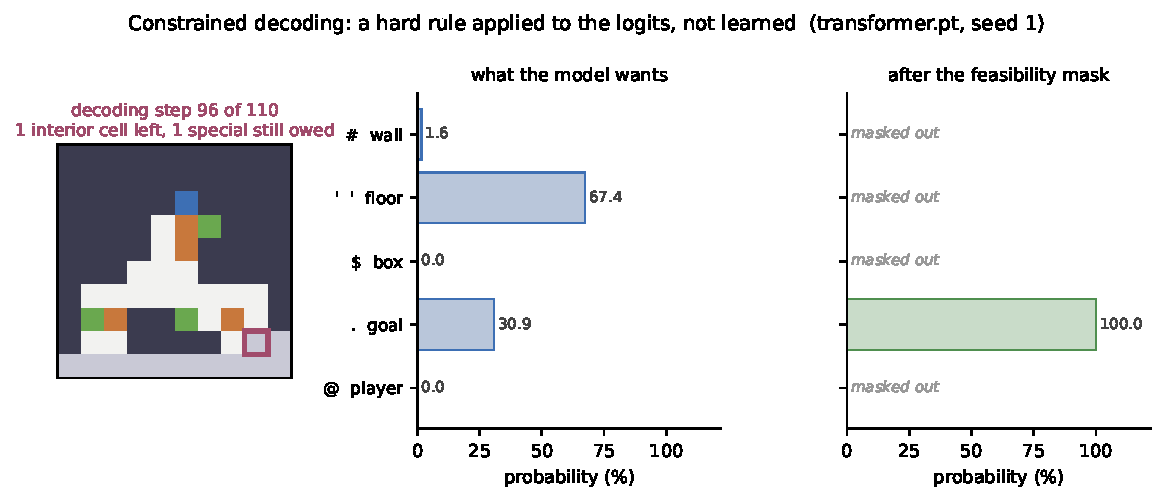
\includegraphics[width=\textwidth]{figures/r3_constrained_decoding.pdf}
\caption[Constrained decoding at a step where it binds]{Feasibility forcing
caught in the act, using the trained checkpoint and real model probabilities. At
decoding step $96$ the model would put $67.4\%$ of its probability mass on
``floor'' and only $30.9\%$ on ``goal''. But one interior cell remains and one
goal is still owed, so the mask removes wall, floor, box and player, and the
renormalised distribution puts $100\%$ on ``goal''. The pale grey region is the
part of the grid not yet emitted; the outlined cell is the one being decided.}
\label{fig:constrained}
\end{figure}

\subsection{How often does it actually fire?}

Because the rule is instrumented, the \textbf{forced-token rate} is a free
measurement of how well the model learned to count on its own. Across the
primary transformer's evaluation sweep, feasibility forcing fired on
\textbf{$25.0\%$ of levels} and supplied a mean of only \textbf{$0.378$ forced
tokens per level} out of $110$. Quota masking touched $34.4$ tokens per level on
average, but quota masking is the cheap half of the rule.

The interpretation is that the model had largely learned to count unaided;
forcing supplies the last box.

\subsection{The honest cost}

Mask-then-renormalise at each step does \emph{not} sample from the model's true
distribution conditioned on the valid set. It is a greedy local approximation to
it, and it therefore shifts the sampling distribution. Section~\ref{sec:invert}
shows this cost appearing as a measurable drop in solvability, which is exactly
why both the constrained and unconstrained rows are reported.

\section{Repair: projecting an invalid grid onto a valid one}

The one-shot models cannot use a per-step mask, because there are no steps.
Instead,
any structurally invalid grid is \textbf{projected onto the nearest valid grid
using the model's own predicted probabilities}:

\begin{enumerate}[leftmargin=1.5em,itemsep=1pt]
\item Force the border to wall.
\item Drop excess boxes, goals and players lowest-probability-first.
\item Fill deficits highest-probability-first.
\item Never place a special tile on the border.
\end{enumerate}

Repair is idempotent and is the identity on already-valid grids.

\keyfinding{Repair is what makes the comparison interpretable. Post-repair
solvability answers ``does this model understand spatial structure?'' while
structural validity answers ``can this model count?'' Without repair, a reader
cannot tell whether the GAN is bad at Sokoban or merely bad at arithmetic,
and as Section~\ref{sec:invert} shows, the answer is not the one the raw numbers
suggest.}

% =====================================================================
\chapter{Evaluation Methodology}
\label{ch:eval}

\section{The solver as a decision procedure}

Every number in this report ultimately comes from the solver, so the solver is
validated before anything else is believed.

Levels are represented as integer bitmasks (walls, goals, boxes) plus a single
player cell index. Successors are \textbf{pushes}, not single steps. For state
hashing the player's exact cell is irrelevant and only its reachable region
matters, so the state key is (minimum reachable cell, box mask). Without this
canonicalisation, states differing only by player position within one region are
distinct and the search inflates by roughly the region size; measured on the
$1{,}000$ real test levels, the starting region averages $19.1$ cells.

The heuristic precomputes, per goal, a backward breadth-first map of the minimum
number of pushes needed to bring a box to that goal, ignoring other boxes but
respecting walls, and then takes the minimum-cost assignment of boxes to
goals. It is admissible, because each push moves one box one cell, and strictly
tighter than sum-of-Manhattan because it respects walls.

\subsection{Two sound prunes, and nothing else}

\begin{itemize}[leftmargin=1.5em,itemsep=2pt]
\item A cell is \textbf{dead} if a box placed there can reach no goal under the
      relaxation above. A box on a dead square is a proven deadlock. This
      subsumes ordinary corner deadlocks.
\item A box is \textbf{frozen} if it is blocked along both axes, where a blocker
      is a wall, a dead square, or another frozen box. A frozen box that is not
      on a goal is a proven deadlock.
\end{itemize}

Nothing heuristic is admitted. An unsound prune produces \emph{false proofs of
unsolvability}, which is the worst failure mode available here: it corrupts the
headline number invisibly, and in the direction that flatters it.

\keyfinding{\texttt{unsolvable} is returned \textbf{only} when the open set
empties before any budget is hit. Every cap hit is reported as
\texttt{timeout}. Collapsing ``timed out'' into ``unsolvable'' would convert an
absence of evidence into a false proof.}

\section{Solver validation}

\begin{table}[!htb]
\centering\small
\caption[Solver validation]{Solver validation, run before any model was evaluated
(\texttt{results/solver\_validation.json}). Node cap $200{,}000$, wall-clock cap
$10$\,s.}
\label{tab:solver}
\begin{tabularx}{\textwidth}{@{}X l@{}}
\toprule
\textbf{Check} & \textbf{Result} \\
\midrule
Solve rate on $1{,}000$ real held-out test levels & \textbf{$100.00\%$} \\
False ``unsolvable'' verdicts on real levels & \textbf{$0$} \\
Returned solutions that replay to a solved state & \textbf{$1000/1000$} \\
Soundness ablation (both prunes disabled, $10\times$ node cap, $200$ levels) &
  \textbf{$0$} verdict and $0$ length disagreements \\
Same ablation on three baseline distributions ($450$ levels) & \textbf{$0$}
  disagreements \\
Push length vs published solutions ($926$ comparable levels) &
  ours $\leq$ theirs on $926/926$ \\
Median / p99 nodes expanded & $176$ / $3{,}458$ \\
Median / p99 wall-clock time & $66$\,ms / $1.4$\,s \\
\bottomrule
\end{tabularx}
\end{table}

The soundness ablation is the check that matters most. It re-runs the search with
both prunes \emph{disabled} and a ten-times larger node budget, and compares
verdicts. Zero disagreements means the prunes never discarded a state that
mattered. It was extended to $450$ levels drawn from the three baseline
generators, whose wall densities and failure modes differ sharply from real
levels, again with zero disagreements.

\begin{figure}[!htb]
\centering
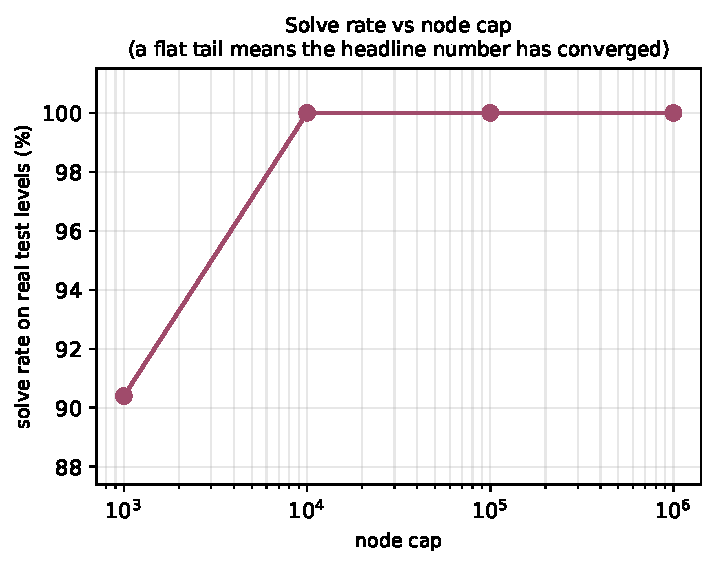
\includegraphics[width=0.60\textwidth]{../figures/figA_node_cap_sensitivity.pdf}
\caption[Node-cap convergence]{The results are converged, not budget-limited. At
a node cap of $1{,}000$ the solver still times out on $9.6\%$ of real levels; at
$10{,}000$ it reaches $100\%$, and it stays flat all the way to $1{,}000{,}000$.
Every headline number in this report uses a cap of $200{,}000$, comfortably
inside the flat region.}
\label{fig:nodecap}
\end{figure}

\subsection{Reconstructed move length is an upper bound}

Because push-optimal search discards the player's exact position, the move
length reconstructed by walking the player between consecutive pushes is an
\emph{upper bound}, not the optimum. Measured against exact move-optimal search
on $196$ levels: mean excess \textbf{$+40.5\%$}, exactly optimal on only $6.6\%$
of levels, and \emph{zero} bound violations.

That gap is far too large to ignore, so the achieved solution length used in the
controllability metric is measured with the \textbf{exact move-optimal solver},
matching the move units used in the captions, rather than with the cheap
reconstruction.

\section{Metrics}

\begin{table}[!htb]
\centering\small
\caption{The metrics used throughout Chapter~\ref{ch:results}.}
\label{tab:metrics}
\begin{tabularx}{\textwidth}{@{}l X@{}}
\toprule
\textbf{Metric} & \textbf{Definition} \\
\midrule
Structural validity \% & Fraction of \emph{raw draws} with a complete wall
border and exactly $(1, 4, 4)$ player, boxes, goals. \\
Solvable \% & Fraction of \emph{all samples drawn} that the solver proves
solvable. \\
Solvable $\mid$ valid \% & Fraction of \emph{structurally valid} samples proven
solvable. Reported separately from validity, never merged. \\
Timeout \% & Fraction on which the solver hit a budget. Never folded into
``unsolvable''. \\
Novelty & Percentage of generated levels that are not an exact copy of any
training level, checked over all $8$ dihedral transforms. \\
NN distance & Mean cell-wise Hamming distance (over $100$ tiles) to the nearest
training level. \\
Diversity & Mean pairwise Hamming distance within the generated set. \\
Controllability & Per attribute: the fraction of samples landing in the caption's
requested bin. For solution length, the Spearman rank correlation between
requested and achieved. \\
\bottomrule
\end{tabularx}
\end{table}

Novelty and diversity are only interpretable against a reference. On $500$
held-out \emph{real} levels the nearest-neighbour distance is $11.92$ and the
diversity is $38.81$; those two numbers anchor every novelty and diversity
figure in this report.

\section{Baselines}

Four non-learned baselines constrain how the headline number may be read. They
are not there to be beaten; they are there to bound the interpretation.

\begin{itemize}[leftmargin=1.5em,itemsep=2pt]
\item \textbf{Random placement.} Uniform interior walls at the training-median
      density, then random special tiles. The floor.
\item \textbf{Open room.} Border walls only, no interior walls at all. This
      baseline exists to \emph{invalidate} the headline number if it can: an
      empty room has no interior walls to freeze a box against, so it should be
      easy to solve.
\item \textbf{Rule-based.} Adds a floor-connectivity check and places boxes
      and goals only on live squares. Hand-written domain knowledge.
\item \textbf{Retrieval.} Samples a training level verbatim. This makes the
      complementary point: solvability alone is trivially maximised by copying.
\end{itemize}

Held-out real Boxoban levels provide the ceiling row.

\section{Statistical protocol}

For each condition we draw until $500$ structurally valid levels are collected,
or until a hard cap of $100{,}000$ draws is reached, and we report
\textbf{samples drawn} as its own column. Only valid samples reach the solver, so
drawing tens of thousands of one-shot samples costs seconds.

\begin{itemize}[leftmargin=1.5em,itemsep=1pt]
\item All proportions carry \textbf{Wilson $95\%$ score intervals}, which behave
      correctly near $0\%$ and $100\%$ where the normal approximation does not.
\item Pairwise comparisons use two-proportion $z$-tests.
\item A ``solvable given valid'' percentage on a denominator below $30$ is
      \textbf{flagged inline as noise}. At $2\%$ validity that denominator is ten
      levels, and a percentage there is noise a reader will misread as signal.
\item Three training seeds are run on the primary transformer and on the
      DistilGPT-2 ablation. \textbf{Every other row is a single run and says so.}
\end{itemize}

Controllability uses a fixed prompt suite stored in the repository: five
solution-length targets $\times$ two density settings $\times$ two connectivity
settings $\times$ two clustering settings $\times$ $15$ samples $= 600$ prompts.
A separate out-of-distribution suite requests $90$, $110$ and $150$ moves.

% =====================================================================
\chapter{Implementation}
\label{ch:impl}

\section{Pipeline}

\begin{figure}[!htb]
\centering
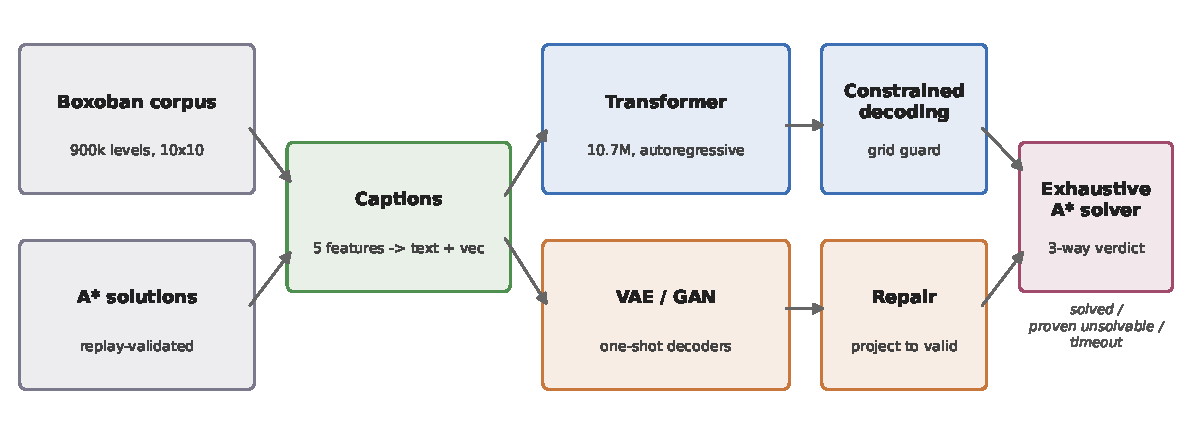
\includegraphics[width=\textwidth]{../figures/fig1_pipeline.pdf}
\caption[System pipeline]{The full system. Levels and replay-validated A*
solutions feed a caption builder that emits both a text caption and a
$10$-dimensional vector. The autoregressive branch generates cell by cell and
passes through constrained decoding; the one-shot branch decodes in a single
step and passes through repair. Everything converges on the exhaustive solver,
which returns one of three verdicts.}
\label{fig:pipeline}
\end{figure}

\section{Stack and hardware}

Python 3.13 with PyTorch (CUDA), \texttt{transformers} for the DistilGPT-2
ablation, NumPy, SciPy and Matplotlib. All training and sampling ran on a single
\textbf{NVIDIA RTX 3050 laptop GPU with 6\,GB of VRAM}, in bf16 mixed precision.
The solver is pure Python operating on integer bitmasks, parallelised across CPU
workers; the full evaluation sweep over $18$ conditions took $1{,}338$ seconds.

Model sizes were chosen to fit that budget honestly. The DistilGPT-2 ablation
uses batch size $32$ rather than $64$ purely because $43$M parameters do not fit
alongside $10.7$M-scale activations on a 6\,GB card.

\section{Repository layout}

\begin{table}[!htb]
\centering\small
\caption{Module layout.}
\label{tab:layout}
\begin{tabularx}{\textwidth}{@{}l X@{}}
\toprule
\texttt{sokogen/data/} & Boxoban parsing, replay-validated solutions, caption
construction, vocabulary. \\
\texttt{sokogen/solver/} & Bitmask grids, sound deadlock detection, exhaustive
A*. \\
\texttt{sokogen/models/} & From-scratch transformer, conditional VAE,
conditional GAN, DistilGPT-2 adapter. \\
\texttt{sokogen/decoding/} & Constrained decoding (the grid guard) and repair. \\
\texttt{sokogen/baselines/} & Random, open room, rule-based, retrieval. \\
\texttt{sokogen/eval/} & Metrics, evaluation harness, tables, figures. \\
\texttt{scripts/} & \texttt{00}--\texttt{07}: the full pipeline in order. \\
\texttt{results/} & JSON artifacts, generated levels with per-level solver
verdicts, tables. \\
\bottomrule
\end{tabularx}
\end{table}

\section{Reproducibility}

The pipeline runs as a fixed sequence of gated scripts:

\begin{center}
\colorbox{softgrey}{\parbox{0.9\textwidth}{\ttfamily\footnotesize
python scripts/00\_verify\_data.py \hfill \# GATE 1: verify every data assumption\\
python scripts/01\_build\_dataset.py \hfill \# GATE 3: captions and datasets\\
python scripts/02\_validate\_solver.py \hfill \# GATE 2: solver + soundness ablation\\
python scripts/03\_train.py -{}-model \{transformer,vae,gan,distilgpt2\}\\
python scripts/04\_generate.py \hfill \# GPU sampling\\
python scripts/05\_evaluate.py \hfill \# CPU solver sweep $\rightarrow$ tables + figures\\
python scripts/06\_seed\_variance.py \hfill \# three seeds per arm\\
python scripts/07\_verify\_paper.py \hfill \# re-derive every quoted number
}}
\end{center}

Seed $1337$ is used throughout and every script accepts \texttt{-{}-seed}. Every
result JSON embeds its configuration, its seed and the git commit SHA that
produced it, and every table in this report is regenerated from those artifacts.

\keyfinding{\texttt{07\_verify\_paper.py} re-derives every numeric claim in the
accompanying manuscript directly from the committed artifacts and fails if any
one of them disagrees. It currently reports \textbf{$108/108$ claims verified}.
The same discipline governs this report: no number appears here that is not
traceable to a JSON artifact under \texttt{results/}.}

\section{Testing}

The solver tests were written \emph{before} the solver. They include roughly
eleven hand-built fixtures with known verdicts and exact push-optimal lengths,
differential testing against an independently written reference solver that
shares no code and no representation, and a check that every ``solved'' verdict
comes with an action string that replays to a solved state.

One operational note recorded during the work is worth repeating: the evaluation
sweep must not be run while a GPU job is active. The GPU heats the package, CPU
cores throttle, and solver throughput silently halves mid-sweep, corrupting
the timing measurements without producing any error.

% =====================================================================
\chapter{Results and Discussion}
\label{ch:results}

Eighteen conditions were sampled and solved. We read the results as six
findings.

\begin{figure}[!htb]
\centering
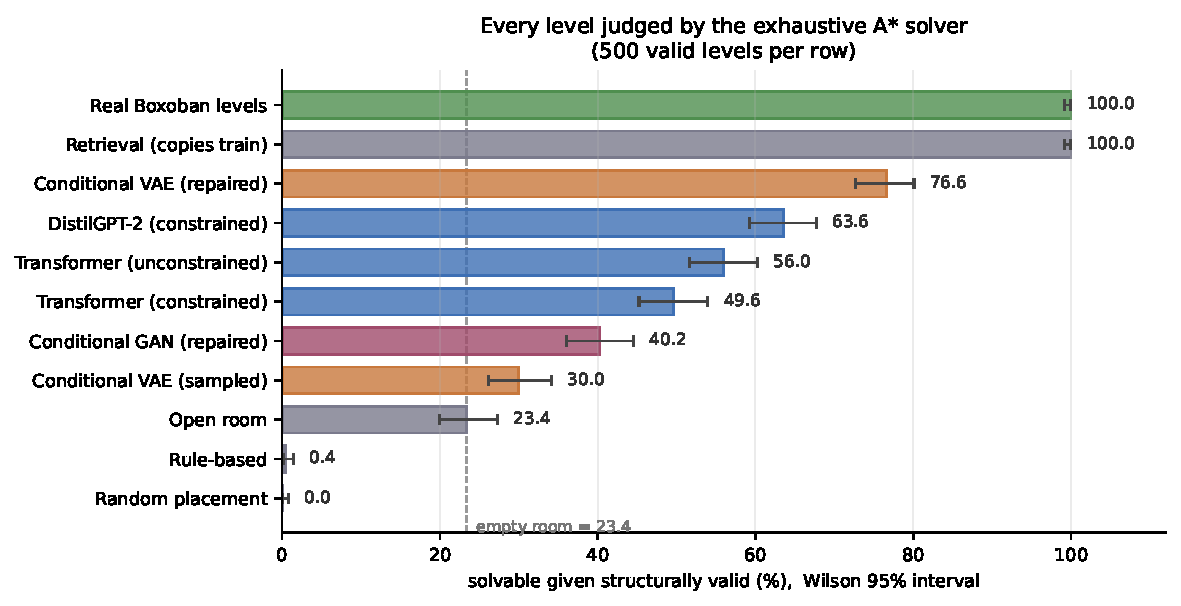
\includegraphics[width=0.98\textwidth]{figures/r5_headline.pdf}
\caption[Headline solvability ranking]{Solvability of every condition, judged by
the exhaustive solver on $500$ structurally valid levels each. The dashed line
is the empty-room baseline. Two rows at $100\%$ are not achievements: retrieval
copies training levels verbatim, and ``real Boxoban levels'' is the ceiling.}
\label{fig:headline}
\end{figure}

\section{Main results}

\begin{table}[!htb]
\centering\footnotesize
\caption[Main results: validity and solvability]{Main results, part 1:
validity and solvability. Percentages carry Wilson $95\%$ intervals. Structural
validity and solvability are reported separately and \textbf{never merged}.
\emph{Every row is a single training run}; see Section~\ref{sec:seeds} for what
that licenses.}
\label{tab:main1}
\begin{tabular}{@{}l r r r r r@{}}
\toprule
\textbf{Model} & \textbf{Struct.} & \textbf{Solvable} &
\textbf{Solvable} & \textbf{Time-} & \textbf{Draws for} \\
& \textbf{valid \%} & \textbf{\%} & $\mid$ \textbf{valid \%} &
\textbf{out \%} & \textbf{500 valid} \\
\midrule
Random placement & $100.0$ & $0.0$ & $0.0$ & $0.0$ & $512$ \\
Open room & $100.0$ & $23.4$ & $23.4$ {\scriptsize[19.9, 27.3]} & $0.0$ & $512$ \\
Rule-based & $100.0$ & $0.4$ & $0.4$ & $0.0$ & $512$ \\
Retrieval & $100.0$ & $100.0$ & $100.0$ & $0.0$ & $512$ \\
\midrule
Cond.\ GAN (raw) & $8.6$ {\scriptsize[8.0, 9.4]} & $4.3$ & $50.2$
  {\scriptsize[45.8, 54.6]} & $0.0$ & $6{,}144$ \\
Cond.\ GAN (repaired) & $100.0$ & $40.2$ & $40.2$ {\scriptsize[36.0, 44.6]} &
  $0.0$ & $512$ \\
Cond.\ VAE (argmax) & $\mathbf{0.0}$ & n/a & n/a & n/a &
  $\mathbf{100{,}000}$ \\
Cond.\ VAE (sampled) & $1.7$ {\scriptsize[1.6, 1.9]} & $0.5$ & $30.0$
  {\scriptsize[26.1, 34.2]} & $0.0$ & $29{,}184$ \\
Cond.\ VAE (repaired) & $100.0$ & $76.6$ & $\mathbf{76.6}$
  {\scriptsize[72.7, 80.1]} & $0.0$ & $512$ \\
\midrule
Transformer (unconstrained) & $\mathbf{82.6}$ {\scriptsize[80.2, 84.8]} &
  $46.3$ & $56.0$ {\scriptsize[51.6, 60.3]} & $0.0$ & $1{,}024$ \\
Transformer (constrained) & $100.0$ & $49.6$ & $49.6$
  {\scriptsize[45.2, 54.0]} & $0.0$ & $512$ \\
DistilGPT-2 (constrained) & $100.0$ & $63.6$ & $63.6$
  {\scriptsize[59.4, 67.8]} & $0.0$ & $512$ \\
\midrule
Real Boxoban levels & $100.0$ & $100.0$ & $100.0$ & $0.0$ & $512$ \\
\bottomrule
\end{tabular}
\end{table}

\begin{table}[!htb]
\centering\footnotesize
\caption[Main results: novelty, diversity and cost]{Main results, part 2:
novelty, diversity and cost. Reference distributions on $500$ held-out real
levels: nearest-neighbour distance $11.92$, diversity $38.81$. Novelty and
diversity are only interpretable against those two numbers.}
\label{tab:main2}
\begin{tabular}{@{}l r r r r r@{}}
\toprule
\textbf{Model} & \textbf{Novel \%} & \textbf{NN dist.} &
\textbf{Diversity} & \textbf{Params} & \textbf{Train (s)} \\
\midrule
Random placement & $100.0$ & $23.97$ & $39.20$ & n/a & n/a \\
Open room & $100.0$ & $20.78$ & $16.22$ & n/a & n/a \\
Rule-based & $100.0$ & $21.55$ & $38.14$ & n/a & n/a \\
Retrieval & $\mathbf{0.0}$ & $\mathbf{0.00}$ & $38.73$ & n/a & n/a \\
\midrule
Cond.\ GAN (raw) & $100.0$ & $11.63$ & $34.18$ & $1{,}082{,}357$ & $153$ \\
Cond.\ GAN (repaired) & $100.0$ & $12.60$ & $36.79$ & $1{,}082{,}357$ & $153$ \\
Cond.\ VAE (argmax) & n/a & n/a & n/a & $1{,}098{,}292$ & $98$ \\
Cond.\ VAE (sampled) & $100.0$ & $12.84$ & $38.54$ & $1{,}098{,}292$ & $98$ \\
Cond.\ VAE (repaired) & $100.0$ & $11.08$ & $37.82$ & $1{,}098{,}292$ & $98$ \\
\midrule
Transformer (unconstrained) & $100.0$ & $12.65$ & $39.01$ & $10{,}734{,}336$ &
  $661$ \\
Transformer (constrained) & $100.0$ & $12.63$ & $38.86$ & $10{,}734{,}336$ &
  $661$ \\
DistilGPT-2 (constrained) & $100.0$ & $12.18$ & $38.69$ & $43{,}352{,}064$ &
  $4479$ \\
\midrule
Real Boxoban levels & $100.0$ & $11.96$ & $38.76$ & n/a & n/a \\
\bottomrule
\end{tabular}
\end{table}

\section{Finding 1: autoregressive models can count; one-shot decoders cannot}

The counting gap is by far the largest effect in the table, and it is structural
rather than a matter of capacity.

\begin{itemize}[leftmargin=1.5em,itemsep=1pt]
\item The transformer reaches $82.6\%$ structural validity \textbf{with no
      constraint at all}, needing $1{,}024$ draws to yield $500$ valid levels.
\item The conditional VAE under argmax decoding yields \textbf{zero} valid levels
      in $100{,}000$ draws.
\item Sampling the VAE per cell instead of taking the argmax raises validity only
      to $1.7\%$, requiring $29{,}184$ draws.
\item The GAN reaches $8.6\%$, requiring $6{,}144$ draws.
\end{itemize}

The tile-count histograms show \emph{why}, far more convincingly than any
percentage can.

\begin{figure}[!htb]
\centering
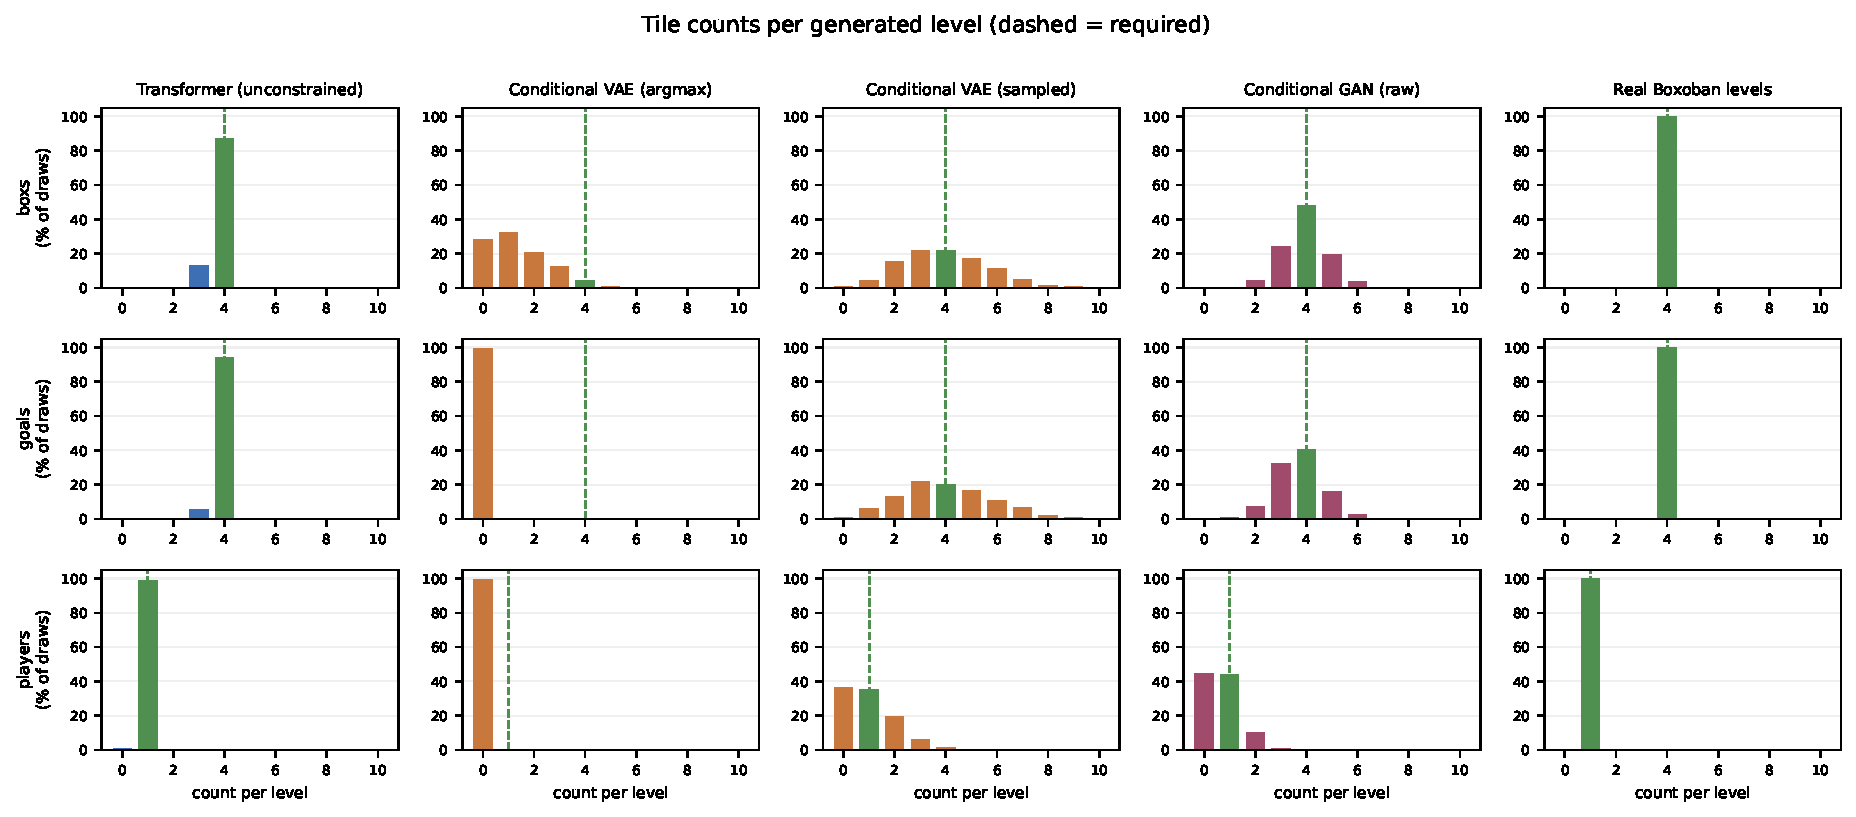
\includegraphics[width=\textwidth]{../figures/fig3_tile_counts.pdf}
\caption[Tile counts per family]{Tile counts per generated level, computed over
\textbf{raw draws, valid or not}; restricting to valid levels would define
the counting failure away. The dashed line marks the required count. The
transformer's distribution is a spike at four. The VAE under argmax collapses to
a near-empty room. VAE sampling recovers the right marginal rate with the wrong
joint.}
\label{fig:tiles}
\end{figure}

\keyfinding{The numbers behind that figure are the clearest statement of the
hypothesis. The transformer: $87.1\%$ of raw draws carry exactly four boxes,
mean $3.87 \pm 0.34$. The VAE under argmax: mean $1.38 \pm 1.23$ boxes and
$0.01 \pm 0.12$ goals, because the per-cell argmax of a product of marginals
picks
floor or wall almost everywhere, because boxes occupy $4/100$ cells. VAE
sampling restores the marginal rates almost exactly (mean $3.95 \pm 1.72$ boxes,
$4.05 \pm 1.85$ goals) but only $21.8\%$ of samples carry exactly four:
\textbf{the right average, the wrong joint}.}

Constrained decoding closes the gap deterministically at $100\%$ validity, and
with a very light touch: feasibility forcing fires on $25.0\%$ of levels and
supplies a mean of $0.378$ forced tokens. The model had largely learned to count;
forcing supplies the last box.

\begin{figure}[!htb]
\centering
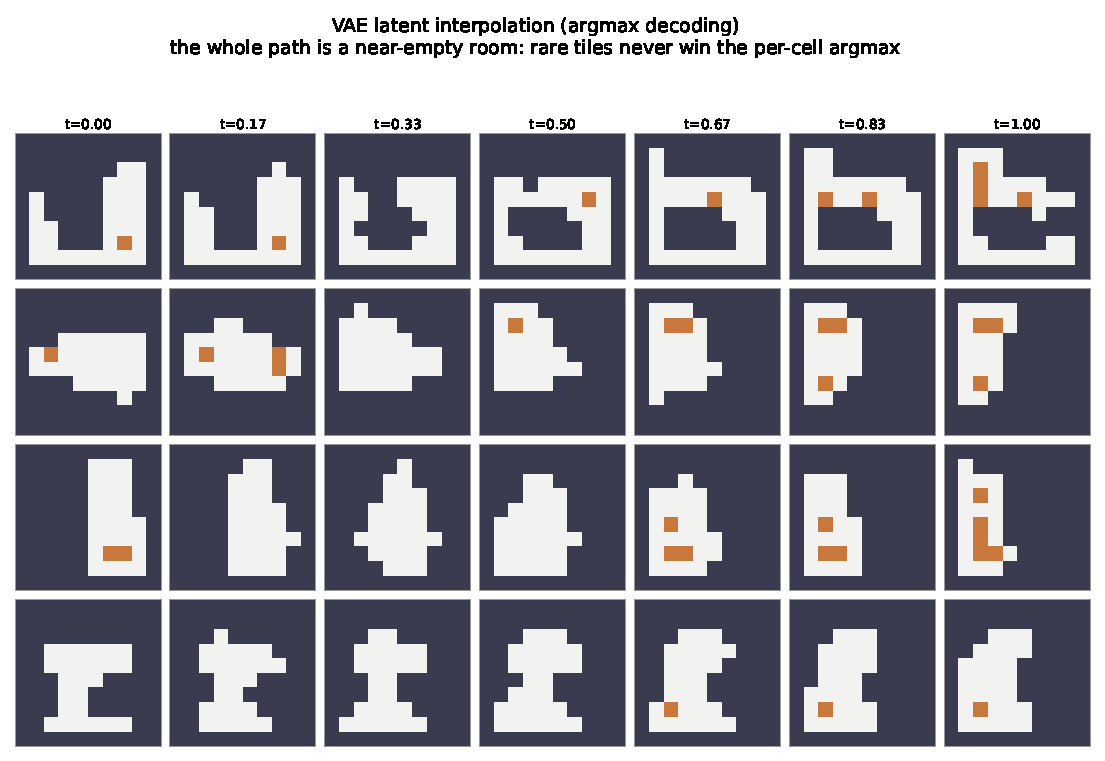
\includegraphics[width=0.78\textwidth]{../figures/figC_vae_interpolation.pdf}
\caption[VAE latent interpolation under argmax]{What the failure actually looks
like. Each row interpolates between two points in the VAE's latent space and
decodes by argmax. The whole path is a plausible, clean, \emph{empty} room,
with one or two boxes at most and no goals at all. The model is not producing noise;
it is producing something that looks like a level and contains no puzzle.}
\label{fig:interp}
\end{figure}

\section{Finding 2: solvability does not follow from validity}

Every non-learned baseline is $100\%$ structurally valid by construction and
still nearly worthless. Random placement is solvable $0.0\%$ of the time and the
rule-based generator $0.4\%$, despite the latter enforcing floor connectivity
and placing boxes only on live squares.

Interior walls are what kill them. At the training-median wall density the floor
becomes a maze of narrow corridors, and a box pushed into one freezes against
the walls.

\begin{figure}[!htb]
\centering
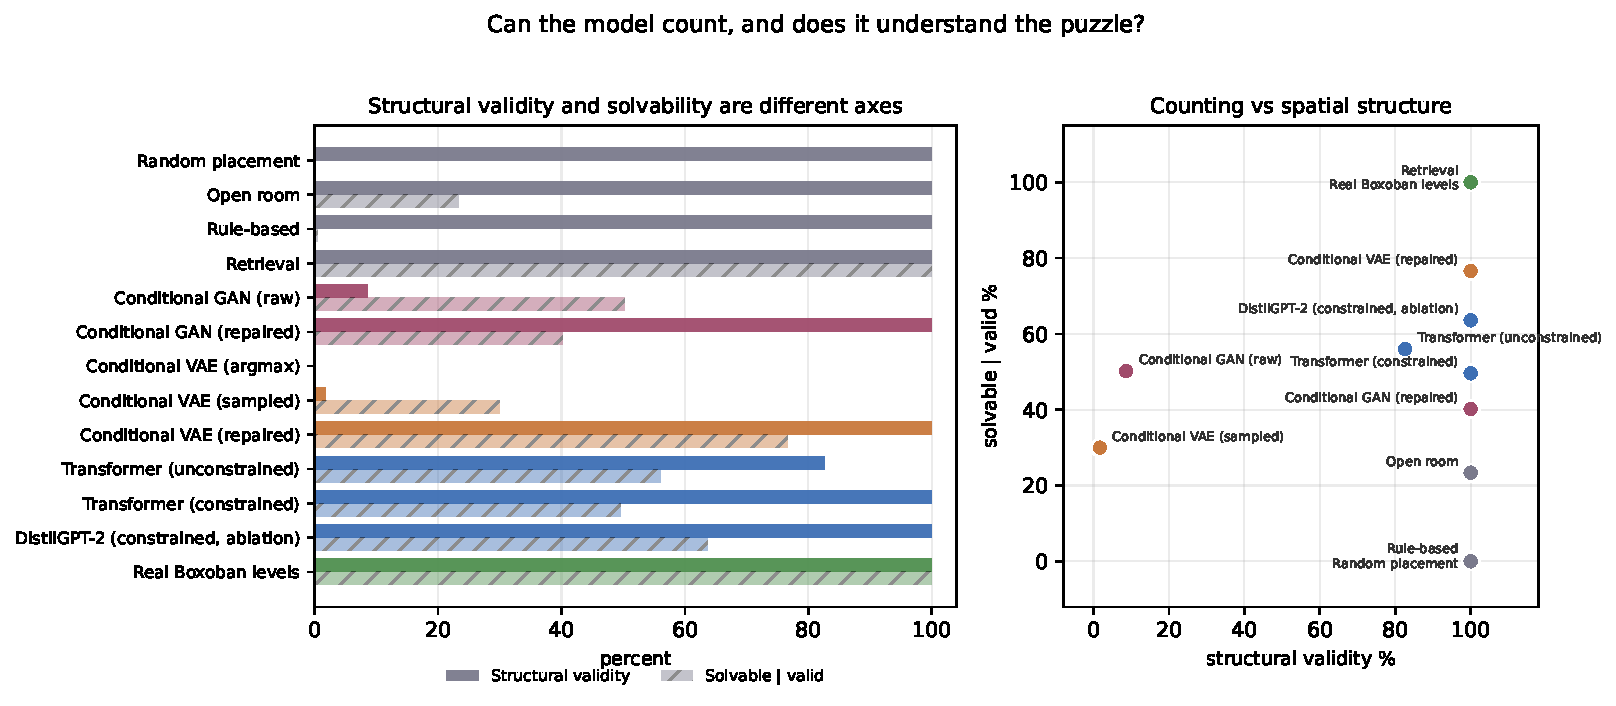
\includegraphics[width=\textwidth]{../figures/fig2_validity_vs_solvability.pdf}
\caption[Validity and solvability are different axes]{\emph{Left:} structural
validity (solid) and solvability given validity (hatched) side by side.
\emph{Right:} the same data as a scatter. The one-shot families sit at the far
left, because they cannot count, while reaching solvability comparable to the
transformer once they are valid. A family can be strong on one axis and weak on
the other, which is why the two are never merged into a single number.}
\label{fig:money}
\end{figure}

The \textbf{open-room} baseline constrains how the headline number may be read.
With no interior walls at all it is already solvable $23.4\%$ of the time. The
transformer's $49.6\%$ is significantly higher, by $+26.2$ points
($z = 8.60$, $p < 10^{-16}$), so the headline is not an artifact of an easy
task. But a reader given only ``$49.6\%$ solvable'' would substantially
overestimate what has been shown.

The \textbf{retrieval} baseline makes the complementary point: $100\%$ solvable,
$0\%$ novel, nearest-neighbour distance exactly $0.00$.

\keyfinding{Solvability alone is a degenerate objective, maximised by copying.
The results table must be read as a \textbf{joint constraint} over solvability,
difficulty control and novelty, never as a single ranking.}

\begin{table}[!htb]
\centering\small
\caption{Pairwise two-proportion $z$-tests on solvable $\mid$ valid.}
\label{tab:sig}
\begin{tabular}{@{}l r r l@{}}
\toprule
\textbf{Comparison} & \textbf{Diff.\ (pp)} & $z$ & $p$ \\
\midrule
Transformer (constr.) vs Open room & $+26.2$ & $8.60$ & $<10^{-16}$ \\
Transformer (constr.) vs Rule-based & $+49.2$ & $17.97$ & $<10^{-16}$ \\
Transformer (constr.) vs Transformer (unconstr.) & $-6.4$ & $-2.03$ &
  $4.27\times10^{-2}$ \\
Transformer (unconstr.) vs Cond.\ VAE (sampled) & $+26.0$ & $8.30$ &
  $<10^{-16}$ \\
Transformer (constr.) vs Real Boxoban levels & $-50.4$ & $-18.35$ &
  $<10^{-16}$ \\
\bottomrule
\end{tabular}
\end{table}

\section{Finding 3: repair separates counting from spatial understanding}
\label{sec:invert}

The most surprising row in the whole table is the repaired VAE. Projecting its
invalid output onto the nearest valid grid yields $76.6\%$ solvability, well
\emph{above} the transformer's $49.6\%$, with diversity ($37.8$) close to the
real-level reference ($38.8$) and no exact copies. The repaired GAN reaches
$40.2\%$.

\keyfinding{\textbf{The VAE is not bad at Sokoban. It is bad at arithmetic.} Its
per-cell marginals already encode where boxes and goals plausibly go; repair
simply reads them off and places the right \emph{number} of tiles at the most
probable positions. What autoregressive generation buys is the ability to
satisfy a counting constraint \emph{while sampling}, not a better model of
spatial structure. Merging validity and solvability into one number would have
hidden this result entirely.}

A second, smaller inversion points the same way. The \emph{unconstrained}
transformer is more solvable given validity ($56.0\%$) than the constrained one
($49.6\%$; $z = -2.03$, $p = 0.043$). The explanation is selection:
unconstrained sampling keeps only the $82.6\%$ of levels the model got right
unaided, which are its more typical and more solvable outputs. Constrained
decoding additionally rescues the levels it would have botched, and those are
worse levels. This is exactly the distribution shift predicted in
Section~\ref{ch:decoding} appearing as a measurable cost, and it is why both
rows are reported. On the overall rate, solvable out of \emph{all} samples
drawn, constrained decoding still wins, $49.6\%$ against $46.3\%$.

\begin{figure}[!htb]
\centering
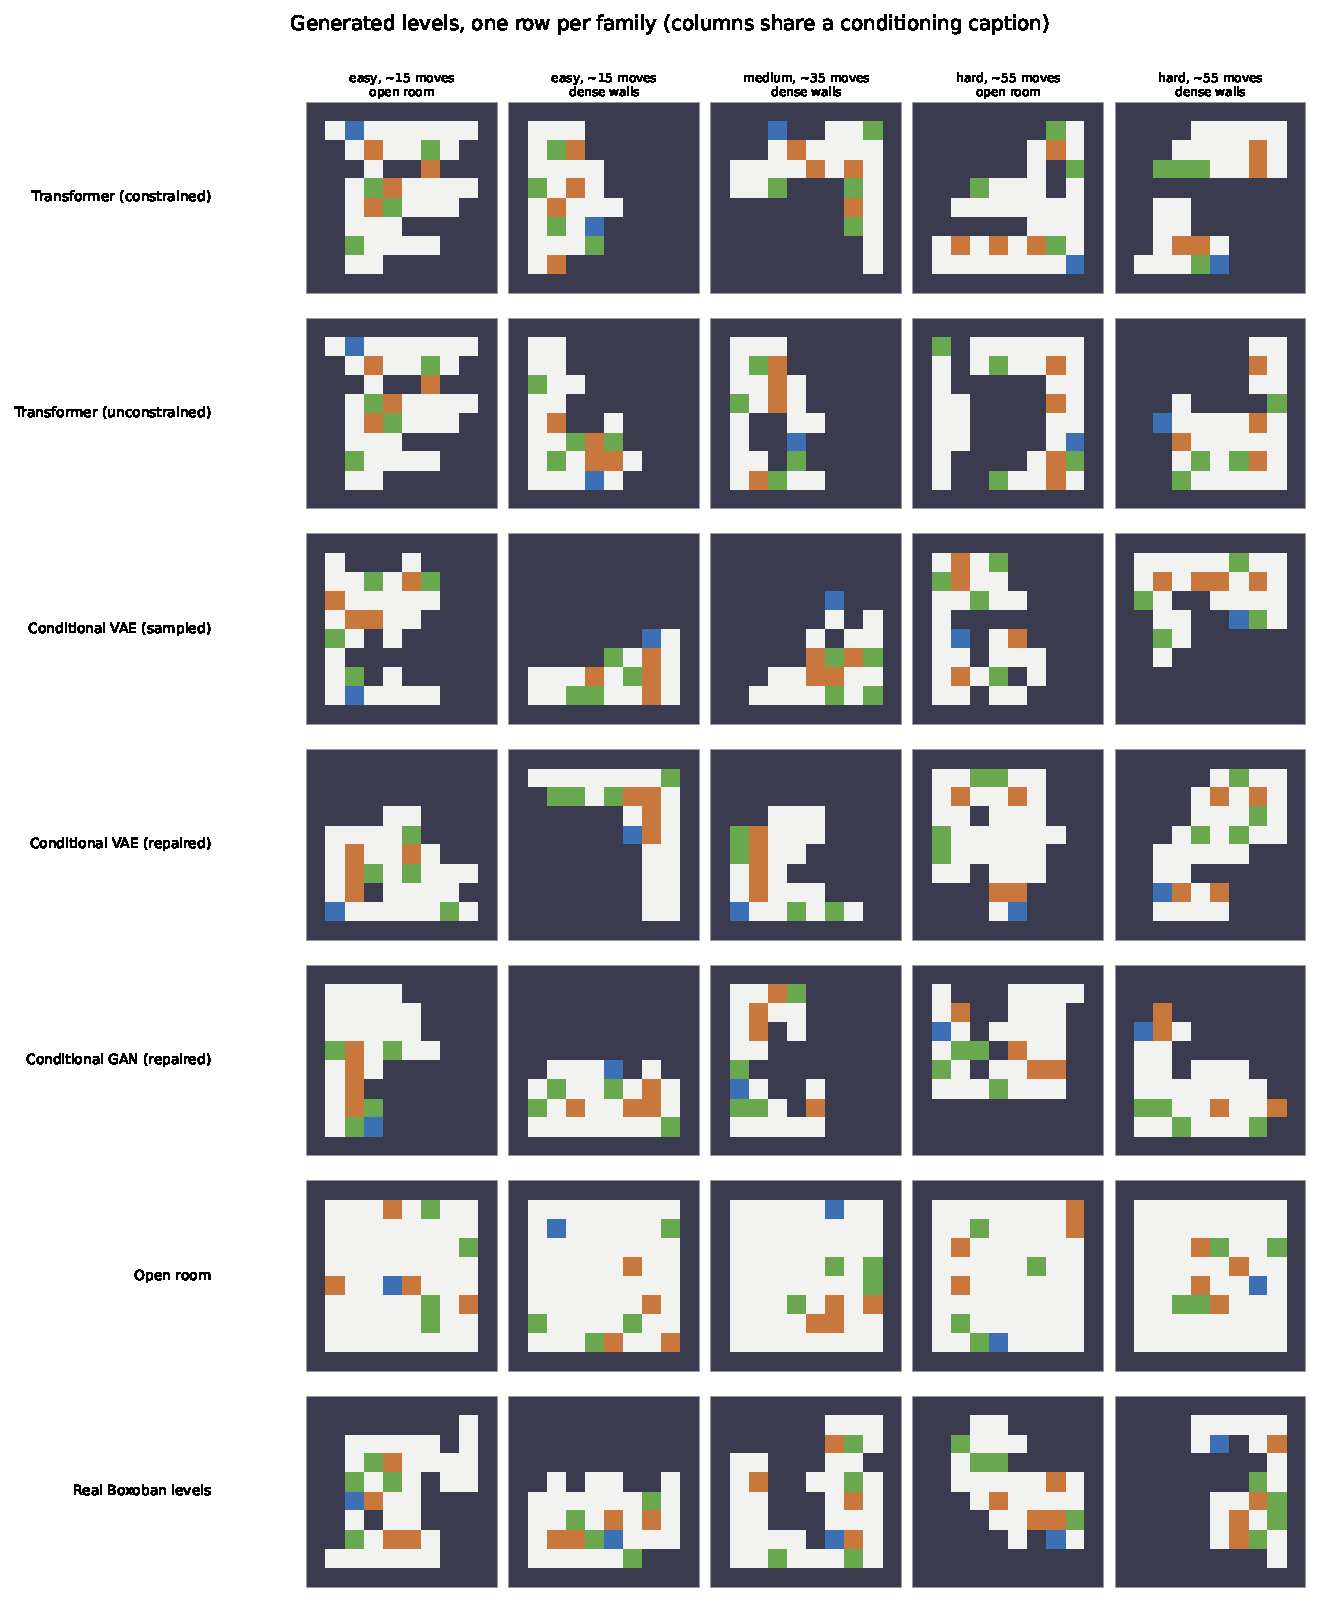
\includegraphics[width=0.63\textwidth]{../figures/fig4_qualitative.pdf}
\caption[Generated levels, one row per family]{Generated levels, one row per
family; columns share a conditioning caption. Note the open-room row, which is
what a $23.4\%$ solvability baseline actually looks like, and the bottom row of
real levels for comparison.}
\label{fig:qual}
\end{figure}

\section{Finding 4: controllability splits along a predictable line}

Control is reported per attribute, never as a single number, and the split is
sharp.

\begin{table}[!htb]
\centering\small
\caption[Controllability per attribute]{Controllability per attribute, for the
key rows. Bin accuracy against a $50\%$ chance rate for the two-bin attributes
and $33\%$ for difficulty. $\rho$ is the Spearman correlation between requested
and achieved solution length.}
\label{tab:control}
\begin{tabular}{@{}l r r r r r r@{}}
\toprule
\textbf{Model} & \textbf{Diffic.} & \textbf{Density} & \textbf{Connect.} &
\textbf{Cluster.} & \textbf{Length} $\rho$ & \textbf{Censor.\ \%} \\
\midrule
Transformer (unconstr.) & $41.3$ & $88.3$ & $84.9$ & $78.6$ & $0.516$ & $47.8$ \\
Transformer (constr.) & $43.3$ & $88.8$ & $80.0$ & $76.3$ & $0.484$ & $55.2$ \\
DistilGPT-2 (constr.) & $53.5$ & $91.5$ & $85.5$ & $86.2$ & $\mathbf{0.673}$ &
  $37.8$ \\
Cond.\ VAE (repaired) & $46.2$ & $88.5$ & $74.2$ & $82.3$ & $0.389$ & $27.0$ \\
Cond.\ GAN (repaired) & $39.0$ & $85.7$ & $64.0$ & $53.8$ & $0.074$ & $59.8$ \\
\midrule
Real levels \emph{(control)} & $31.0$ & $48.8$ & $53.2$ & $52.2$ & $-0.048$ &
  $1.2$ \\
\bottomrule
\end{tabular}
\end{table}

The constrained transformer hits the caption's wall-density bin $88.8\%$ of the
time, connectivity $80.0\%$ and box clustering $76.3\%$, against a $50\%$ chance
rate confirmed by the unconditioned real-level control ($48.8$, $53.2$, $52.2$).
But \textbf{difficulty}, the binned solution length, is hit only $43.3\%$
of the time against a $33\%$ chance rate, with a rank correlation of $0.484$
between requested and achieved length.

\keyfinding{The dividing line was predicted before the experiment ran. Wall
density, connectivity and clustering are \textbf{computable directly from the
grid}, so a model that reproduces surface statistics gets them nearly for free.
\textbf{Solution length is not computable without search.} It is the only
conditioned attribute that requires the model to have learned something about
the \emph{puzzle} rather than about its \emph{pixels}, and it is the one the
model controls worst.}

That correlation is also \textbf{censored}: $55.2\%$ of suite samples have no
achieved length at all, because they were proven unsolvable, and the surviving
subsample is biased toward easy levels, the direction that inflates $\rho$.
The honest reading is that $0.484$ is an \emph{upper bound} on a weak effect.

\section{Finding 5: temperature trades solvability against diversity}

\begin{table}[!htb]
\centering\small
\caption{Temperature sweep on the constrained transformer.}
\label{tab:temp}
\begin{tabular}{@{}l r r r@{}}
\toprule
\textbf{Temperature} & \textbf{Solvable} $\mid$ \textbf{valid \%} &
\textbf{Diversity} & \textbf{Novel \%} \\
\midrule
$0.6$ & $61.2$ {\scriptsize[56.9, 65.4]} & $35.82$ & $100.0$ \\
$0.8$ & $53.8$ {\scriptsize[49.4, 58.1]} & $37.34$ & $100.0$ \\
$1.0$ & $51.4$ {\scriptsize[47.0, 55.8]} & $38.86$ & $100.0$ \\
$1.2$ & $41.4$ {\scriptsize[37.2, 45.8]} & $39.00$ & $100.0$ \\
$1.5$ & $34.8$ {\scriptsize[30.8, 39.1]} & $38.03$ & $100.0$ \\
\bottomrule
\end{tabular}
\end{table}

The trade-off is clean and monotone: solvability falls from $61.2\%$ at
$T = 0.6$ to $34.8\%$ at $T = 1.5$, while diversity rises from $35.8$ to a peak
of $39.0$ at $T = 1.2$. \textbf{$T = 1.5$ is Pareto-dominated}: it loses
solvability without buying diversity back. At $T = 1.0$ the model already matches
the real-level diversity reference ($38.9$ against $38.8$).

\begin{figure}[!htb]
\centering
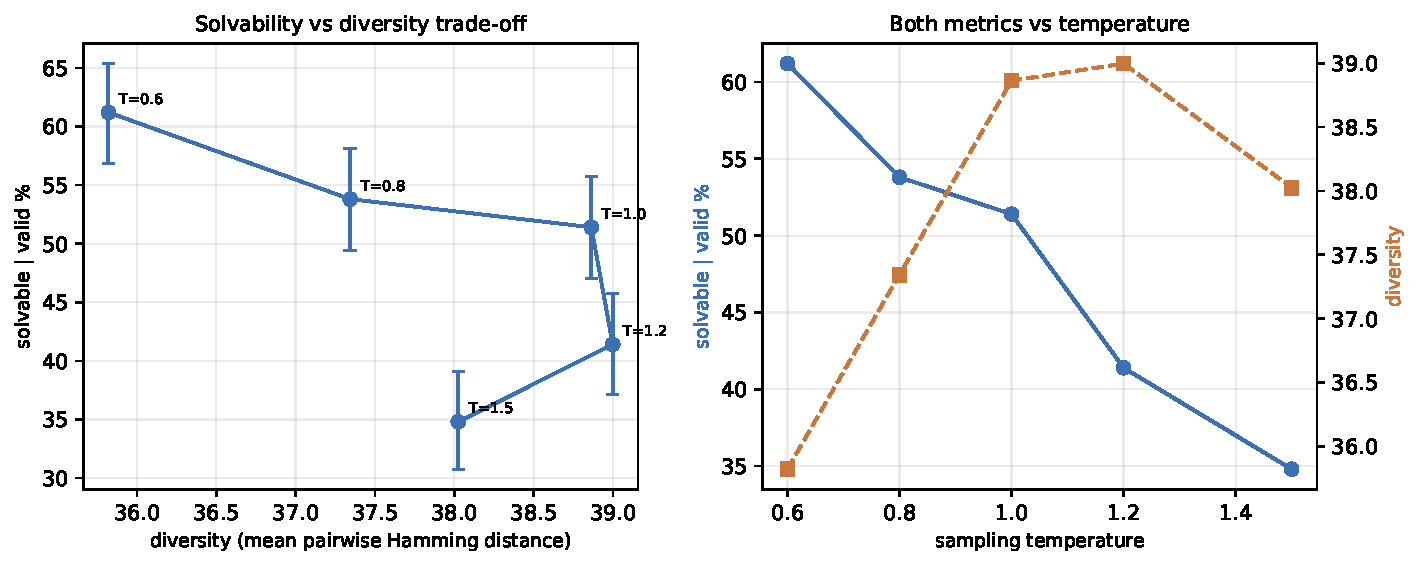
\includegraphics[width=0.60\textwidth]{../figures/fig5_temperature_pareto.pdf}
\caption[Temperature Pareto frontier]{Solvability against diversity across
sampling temperatures. Bars are Wilson $95\%$ intervals. The point at $T = 1.5$
sits inside the frontier.}
\label{fig:pareto}
\end{figure}

\section{Finding 6: seed variance is large, and it bounds every other claim}
\label{sec:seeds}

We trained the primary transformer configuration \textbf{three times}, changing
only the random seed, and sampled and solved each run identically.

\begin{table}[!htb]
\centering\small
\caption[Seed variance]{Three independent training runs per configuration, seed
the only difference. Individual run values in small type.}
\label{tab:seeds}
\begin{tabular}{@{}l l l l@{}}
\toprule
\textbf{Model} & \textbf{Struct.\ valid \%} & \textbf{Solvable} $\mid$
\textbf{valid \%} & \textbf{Validation loss} \\
\midrule
Transformer & $100.0 \pm 0.0$ & $\mathbf{42.7 \pm 7.0}$ &
  $0.3565 \pm 0.0049$ \\
\emph{(primary)} & {\scriptsize $100.0$, $100.0$, $100.0$} &
  {\scriptsize $46.6$, $34.6$, $47.0$} &
  {\scriptsize $0.3546$, $0.3621$, $0.3529$} \\
\addlinespace
DistilGPT-2 & $100.0 \pm 0.0$ & $\mathbf{64.2 \pm 1.8}$ &
  $0.3414 \pm 0.0006$ \\
\emph{(ablation)} & {\scriptsize $100.0$, $100.0$, $100.0$} &
  {\scriptsize $63.6$, $62.8$, $66.2$} &
  {\scriptsize $0.3415$, $0.3407$, $0.3418$} \\
\bottomrule
\end{tabular}
\end{table}

\begin{figure}[!htb]
\centering
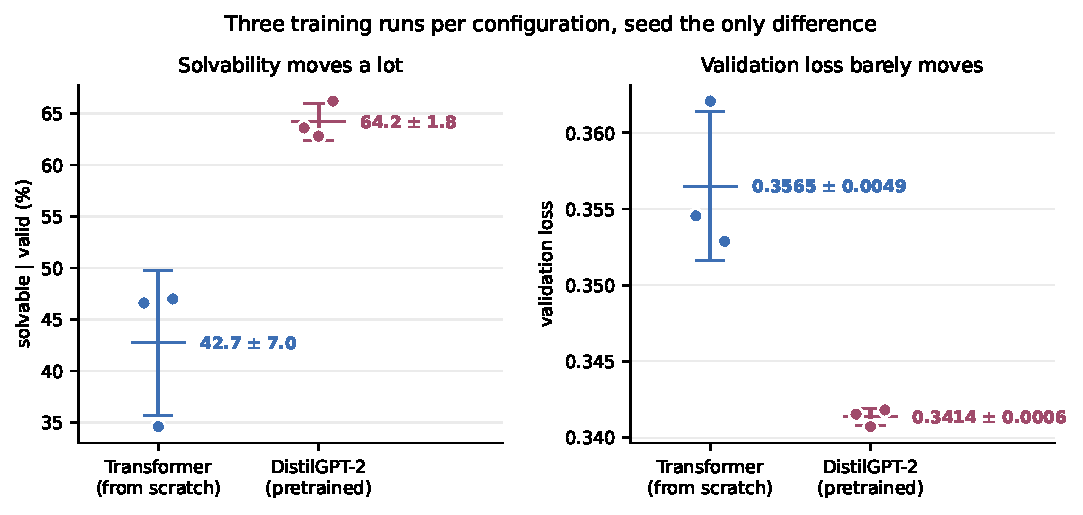
\includegraphics[width=0.92\textwidth]{figures/r4_seed_variance.pdf}
\caption[Seed variance versus validation loss]{The same six training runs viewed
two ways. Solvability, the property we actually care about, moves by
$\pm 7.0$ points for the from-scratch transformer. Validation loss across the
same three runs moves by $\pm 0.005$. The metric that is cheap to measure is not
tracking the metric that matters.}
\label{fig:seeds}
\end{figure}

Structural validity is perfectly stable at $100.0\% \pm 0.0$, unsurprisingly,
since constrained decoding guarantees it, and diversity is stable at
$38.60 \pm 0.31$. Solvability is \textbf{not}: $46.6\%$, $34.6\%$, $47.0\%$.

\keyfinding{\textbf{Validation loss is a poor proxy for the property being
evaluated.} It moves by $\pm 0.005$ across three runs whose solvability moves by
$\pm 7.0$ points. Anyone selecting a checkpoint by validation loss in this
setting is selecting close to at random with respect to playability.}

This number governs how firmly the rest of the table may be read:

\begin{itemize}[leftmargin=1.5em,itemsep=2pt]
\item The comparison against the baselines \textbf{survives easily}. Even the
      worst of the three seeds ($34.6\%$) is far above open room ($23.4\%$) and
      rule-based ($0.4\%$).
\item The constrained-versus-unconstrained gap ($6.4$ points) is \emph{smaller}
      than the seed spread. It is a within-checkpoint decoding comparison, so
      training-seed variance does not apply to it directly, but it is measured on
      one model and should be treated as indicative only.
\item \textbf{Every other row in this report is single-seed.} Given a $\pm 7$
      point spread on the headline metric, no row-to-row difference under roughly
      $15$ points should be read as established without repeated runs.
\end{itemize}

\section{Finding 7: pretraining transfers across a vocabulary boundary}
\label{sec:pretrain}

Because the from-scratch model's own seed spread is $\pm 7.0$ points, a
single-run comparison against DistilGPT-2 would prove nothing. So the ablation
was trained three times as well.

Across three seeds it reaches $\mathbf{64.2\% \pm 1.8}$ solvability against the
from-scratch model's $42.7\% \pm 7.0$, a $21.5$-point gap. \textbf{The two
sets of runs do not overlap at all} ($62.8$--$66.2$ against $34.6$--$47.0$),
which is the strongest separation obtainable from three runs per arm: the exact
permutation test returns $p = 0.05$, its floor at this sample size, and a Welch
$t$-test gives $t = 5.12$, $p = 0.028$.

It also needs less rescuing from the constrained decoder ($10.0\% \pm 3.4$ of
levels against $33.7\% \pm 18.9$) and controls solution length better
($\rho = 0.673$ against $0.484$).

\keyfinding{Pretrained sequence-modelling machinery \textbf{does transfer} to a
domain that shares no vocabulary with the pretraining corpus. The embedding
matrix and LM head were discarded and re-initialised; only attention and MLP
blocks survived, and they were enough.}

A second, unplanned observation is arguably more interesting than the mean
shift: the pretrained model is far more \textbf{stable} across seeds, with a
standard deviation of $1.8$ points against $7.0$, a $4.0\times$ reduction. We
flag this as an \emph{observation}, not a result: with three runs per arm a
variance test has almost no power, and Levene's test is unsurprisingly
inconclusive ($p = 0.50$). If it held up at larger $n$, it would suggest that
part of what pretraining buys here is a better-conditioned \emph{initialisation}
rather than transferred knowledge.

The cost is unambiguous: $4.0\times$ the parameters ($43.4$M against $10.7$M)
and $6.8\times$ the training time ($3897$\,s against $573$\,s, averaged over the
same three runs).

% =====================================================================
\section{Failure analysis: where every family breaks}
\label{ch:failure}

Negative results are reported here as findings. None of them were tuned away.

\subsection{Extrapolation fails completely}

The out-of-distribution suite requests solution lengths of $90$, $110$ and $150$
moves, against a training distribution whose $99$th percentile is $67$ moves and
whose maximum is $130$.

\textbf{Every family ignores the request.}

\begin{table}[!htb]
\centering\small
\caption[Out-of-distribution length requests]{Out-of-distribution requests. The
models produce roughly $30$-move levels when asked for roughly $116$. Real
Boxoban levels sampled against the same captions are the correct null, since
they are not conditioned at all.}
\label{tab:ood}
\begin{tabular}{@{}l r r r r@{}}
\toprule
\textbf{Model} & \textbf{OOD} $\rho$ & \textbf{Censor.\ \%} &
\textbf{Mean requested} & \textbf{Mean achieved} \\
\midrule
Transformer (constr.) & $-0.394$ & $60.0$ & $115.8$ & $29.5$ \\
DistilGPT-2 (constr.) & $-0.274$ & $51.7$ & $120.0$ & $30.4$ \\
Cond.\ VAE (repaired) & $-0.059$ & $55.0$ & $117.8$ & $42.3$ \\
Cond.\ GAN (repaired) & $-0.131$ & $62.5$ & $117.1$ & $24.9$ \\
Real levels \emph{(null)} & $0.131$ & $0.8$ & $116.9$ & $30.3$ \\
\bottomrule
\end{tabular}
\end{table}

The constrained transformer produces levels averaging $29.5$ achieved moves when
asked for $115.8$, with a rank correlation of $-0.394$, pointing the wrong
way. Models reproduce the training length distribution regardless of what the
caption asks for.

\keyfinding{\textbf{Length conditioning learned in-distribution does not extend
past the data.} This is the expected result and we report it as such, but it is
worth stating plainly: a model conditioned on ``$150$ moves'' has learned an
association between a phrase and a region of its training distribution, not a
mechanism for producing long puzzles.}

\subsection{The one-shot failure mode is a plausible, empty room}

The VAE's argmax output is \emph{not} noise. It is a clean, empty, unplayable
room with roughly one box and no goals whatsoever (Figure~\ref{fig:interp}).

It fails the constraint in the most systematic way available, and it fails
\emph{silently}: nothing about the output looks malformed, there is simply no
puzzle in it. A soft metric comparing tile histograms in aggregate would not
obviously flag this, which is a small but real argument for verification over
proxies.

\subsection{Hand-written domain knowledge is not a shortcut}

The rule-based generator, which adds floor-connectivity checks and live-square
placement, achieves $0.4\%$ solvability, \emph{worse than an empty room}. Two
alternative explanations were checked before accepting that number:

\begin{enumerate}[leftmargin=1.5em,itemsep=2pt]
\item \textbf{Is the solver wrong?} No. Re-solving $450$ baseline levels with
      deadlock pruning disabled at a $10\times$ node cap gives identical
      verdicts.
\item \textbf{Do the levels start in a deadlock?} No. Additionally rejecting
      frozen start states moves the rate by less than one point. The levels die
      \emph{after} the first push, not before it.
\end{enumerate}

Real Boxoban levels reach $100\%$ solvability at the same wall density only
because they are built by \textbf{reverse play from an already-solved state},
which is a fundamentally different construction from sampling walls and then
dropping boxes onto them. Domain knowledge applied in the wrong direction buys
nothing.

\subsection{GAN mode collapse}

The GAN's training curves (Figure~\ref{fig:curves}, right) show the generator
loss climbing while the discriminator loss stays flat and low: the
discriminator has won. Its raw structural validity is $8.6\%$ and its
nearest-neighbour distance ($11.63$) sits below the real-level reference
($11.92$), consistent with reduced coverage. The family was hard time-boxed at
three hours and this is reported as an outcome, not repaired.

% =====================================================================
\chapter{Limitations, Ethics and Conclusion}
\label{ch:conclusion}

\section{Limitations}

Stated plainly, because each of these bounds a claim made above.

\begin{itemize}[leftmargin=1.5em,itemsep=3pt]
\item \textbf{Constrained decoding shifts the sampling distribution.}
      Mask-then-renormalise at each step is a greedy local approximation to
      sampling from the model's distribution conditioned on the valid set, not
      the thing itself.
\item \textbf{Conditioning channels differ across families.} The transformer is
      conditioned on caption \emph{text} and the one-shot models on a
      $10$-dimensional \emph{vector}, so the family comparison is not perfectly
      controlled on conditioning.
\item \textbf{Reconstructed move length is an upper bound}, quantified at
      $+40.5\%$ mean excess. We avoid it where it matters by using exact
      move-optimal search for controllability.
\item \textbf{A single game at a single fixed size.} $10\times10$, four boxes,
      four goals. Nothing here shows the finding generalises to other tile games
      or other grid sizes.
\item \textbf{Large seed variance.} Only the transformer and the DistilGPT-2
      ablation were run with three seeds. Every other row is a single run, and
      differences smaller than roughly $15$ points between those rows are
      \emph{not} established.
\item \textbf{Untuned hyperparameters.} Learning rate, batch size and epoch count
      were chosen once and never swept, for any model.
\item \textbf{Inverse-binomial sampling.} Because we draw until $500$ valid
      levels are collected, the structural-validity intervals are close
      approximations rather than exact fixed-$n$ binomial intervals.
\item \textbf{Censored controllability.} Achieved solution length exists only for
      solved levels, so the length correlation is computed on a subsample biased
      toward easy levels. The censoring rate is reported alongside it every time.
\end{itemize}

\section{Ethical considerations}

The models generate puzzle layouts for a single game. They consume no personal
data, produce no text about people, and inform no decisions about people. The
Boxoban corpus is procedurally generated and contains no human-authored or
personal content.

The one substantive risk is \textbf{misreading the verification claim}.
``Solver-verified'' is a strong guarantee \emph{only within stated bounds}: a
$10\times10$ grid, four boxes, a $200{,}000$-node cap and a $10$-second
wall-clock cap. Outside those bounds a timeout proves nothing, which is exactly
why timeouts are a separate column rather than folded into ``unsolvable''.
Presenting a bounded decision procedure as an unbounded guarantee is the failure
mode to avoid.

\section{Conclusion}

We evaluated three generative model families using an exhaustive A* solver as a
decision procedure rather than a proxy, on a solver validated first: $100.00\%$
solve rate on $1{,}000$ real levels, zero false proofs of unsolvability, and
zero verdict disagreements in a soundness ablation across four level
distributions. Three claims hold.

\begin{enumerate}[leftmargin=1.5em,itemsep=3pt]
\item \textbf{Autoregressive generation satisfies counting constraints that
      one-shot decoders cannot}, at $82.6\%$ structural validity unaided against
      \emph{zero} valid levels in $100{,}000$ VAE draws. Constrained decoding
      closes the gap deterministically, and the forced-token rate shows it only
      has to supply the last box.
\item \textbf{Solvability does not follow from validity}, and the open-room
      baseline at $23.4\%$ bounds how much of a headline number comes from the
      task rather than from the model.
\item \textbf{The two axes come apart the other way as well.} Once its counting
      errors are repaired the VAE is \emph{more} solvable ($76.6\%$) than the
      transformer ($49.6\%$), locating the autoregressive advantage in counting
      rather than in spatial understanding.
\end{enumerate}

Measuring across seeds proved essential: solvability moves by $\pm 7.0$ points
across three runs while validation loss moves by $\pm 0.005$, and repeating the
pretraining ablation under the same protocol settles it at $64.2\% \pm 1.8$
against $42.7\% \pm 7.0$ with no overlap between the two sets of runs.

\keyfinding{The most interesting negative result is the controllability split.
Attributes computable from the grid are controlled well; solution length, which
requires search to evaluate, is controlled weakly ($\rho = 0.484$, censored) and
not at all out of distribution. \textbf{A model conditioned on ``hard'' learns
what hard levels \emph{look like}, not what makes them hard}, and that gap is
invisible to any metric that does not run the game.}

\section{Future work}

\begin{itemize}[leftmargin=1.5em,itemsep=2pt]
\item \textbf{Search-in-the-loop training.} The clearest gap is solution-length
      control. Using solver feedback as a training signal, whether rejection
      sampling against a length target or a preference objective over solver
      verdicts, attacks it directly.
\item \textbf{More seeds, fewer claims.} The variance-reduction observation under
      pretraining needs many more than three runs per arm to test properly.
\item \textbf{Matched conditioning channels.} Feeding the one-shot models caption
      \emph{text} through a small encoder would remove the one uncontrolled
      variable in the family comparison.
\item \textbf{Other grid sizes and other tile games}, to test whether the
      counting result is a property of autoregressive decoding in general or of
      this particular grid.
\item \textbf{Exact constrained sampling.} Replacing greedy
      mask-then-renormalise with a method that samples correctly from the
      constrained distribution would remove the measured cost documented in
      Section~\ref{sec:invert}.
\end{itemize}

% =====================================================================
\chapter*{References}
\addcontentsline{toc}{chapter}{References}
\markboth{References}{References}

\begin{enumerate}[leftmargin=2.2em,itemsep=3pt,label={[\arabic*]}]
\item G.\ Todd, S.\ Earle, M.\ U.\ Nasir, M.\ C.\ Green and J.\ Togelius,
      ``Level Generation Through Large Language Models,'' in \emph{Proc.\ 18th
      Int.\ Conf.\ on the Foundations of Digital Games (FDG)}, 2023.
      \emph{The work this project replicates and extends.}
\item S.\ Sudhakaran, M.\ González-Duque, C.\ Glanois, M.\ Freiberger,
      E.\ Najarro and S.\ Risi, ``MarioGPT: Open-Ended Text2Level Generation
      through Large Language Models,'' in \emph{Advances in Neural Information
      Processing Systems}, 2023.
\item A.\ Summerville et al., ``Procedural Content Generation via Machine
      Learning (PCGML),'' \emph{IEEE Trans.\ Games}, vol.\ 10, no.\ 3, 2018.
\item A.\ Guez, M.\ Mirza, K.\ Gregor, R.\ Kabra et al., ``An Investigation of
      Model-Free Planning: Boxoban Levels,''
      \texttt{github.com/google-deepmind/boxoban-levels}, 2018.
      \emph{The level corpus.}
\item A.\ Garriga-Alonso, M.\ Taufeeque and A.\ Gleave, ``Planning behaviour in a
      recurrent neural network that plays Sokoban,'' \emph{ICML 2024 Mechanistic
      Interpretability Workshop}, 2024. \emph{The A* solution set.}
\item S.\ Racanière, T.\ Weber, D.\ Reichert et al., ``Imagination-Augmented
      Agents for Deep Reinforcement Learning,'' in \emph{NeurIPS}, 2017.
      \emph{The level-generation procedure behind Boxoban.}
\item J.\ Culberson, ``Sokoban is PSPACE-complete,'' Technical Report TR97-02,
      University of Alberta, 1997.
\item A.\ Junghanns and J.\ Schaeffer, ``Sokoban: Enhancing General Single-Agent
      Search Methods Using Domain Knowledge,'' \emph{Artificial Intelligence},
      vol.\ 129, 2001.
\item L.\ Orseau, L.\ Lelis, T.\ Lattimore and T.\ Weber, ``Single-Agent Policy
      Tree Search with Guarantees,'' in \emph{NeurIPS}, 2018.
\item M.\ Chen et al., ``Evaluating Large Language Models Trained on Code,''
      arXiv:2107.03374, 2021. \emph{HumanEval; execution-based evaluation.}
\item L.\ de Moura and S.\ Ullrich, ``The Lean 4 Theorem Prover and Programming
      Language,'' in \emph{Int.\ Conf.\ on Automated Deduction}, 2021.
\item T.\ Yu et al., ``Spider: A Large-Scale Human-Labeled Dataset for Complex
      and Cross-Domain Semantic Parsing and Text-to-SQL Task,'' in
      \emph{EMNLP}, 2018.
\item D.\ P.\ Kingma, T.\ Salimans, R.\ Jozefowicz, X.\ Chen, I.\ Sutskever and
      M.\ Welling, ``Improving Variational Inference with Inverse Autoregressive
      Flow,'' in \emph{NeurIPS}, 2016. \emph{Free bits.}
\item E.\ Jang, S.\ Gu and B.\ Poole, ``Categorical Reparameterization with
      Gumbel-Softmax,'' in \emph{ICLR}, 2017.
\item H.\ W.\ Kuhn, ``The Hungarian Method for the Assignment Problem,''
      \emph{Naval Research Logistics Quarterly}, vol.\ 2, 1955.
      \emph{The solver's admissible heuristic.}
\item E.\ B.\ Wilson, ``Probable Inference, the Law of Succession, and
      Statistical Inference,'' \emph{J.\ Amer.\ Statist.\ Assoc.}, vol.\ 22,
      1927. \emph{The confidence intervals used throughout.}
\end{enumerate}

% =====================================================================
\appendix
\titleformat{\chapter}[display]
  {\normalfont\sffamily\bfseries\color{accent}}
  {\filright\normalsize\sffamily\color{rulegrey}APPENDIX \thechapter}
  {4pt}
  {\Large\raggedright}
  [\vspace{2pt}{\color{accent}\titlerule[1.1pt]}]
\chapter{Reproduction and Artifacts}

\section{What is released}

All code, configurations, checkpoints, generated levels \emph{with per-level
solver verdicts}, and result JSON artifacts accompany this report. Every
artifact embeds the configuration, seed and git commit SHA that produced it.

\begin{table}[!htb]
\centering\small
\caption{Result artifacts and what each one backs.}
\label{tab:artifacts}
\begin{tabularx}{\textwidth}{@{}l X@{}}
\toprule
\texttt{data\_verification.json} & Chapter~\ref{ch:data}: the alphabet, invariant
and solution-unit checks. \\
\texttt{dataset\_build.json} & Caption bins, split sizes, class balance. \\
\texttt{solver\_validation.json} & Table~\ref{tab:solver}, the node-cap curve and
the move-bound measurement. \\
\texttt{train\_*.json} & Parameter counts, training times and loss histories for
all four models and all seeds. \\
\texttt{generation.json} & Sampling records for all $18$ conditions. \\
\texttt{evaluation.json} & Every number in Chapter~\ref{ch:results}. \\
\texttt{seed\_variance*.json} & Section~\ref{sec:seeds} and
Section~\ref{sec:pretrain}. \\
\texttt{generated/*.jsonl} & Every generated level with its solver verdict. \\
\bottomrule
\end{tabularx}
\end{table}

\section{Full reproduction}

\begin{center}
\colorbox{softgrey}{\parbox{0.9\textwidth}{\ttfamily\footnotesize
pip install -r requirements.txt\\[2pt]
git clone https://github.com/google-deepmind/boxoban-levels \textbackslash\\
\hspace*{2em}data\_raw/boxoban-levels\\[2pt]
\# then run scripts 00 through 07 in order (see Chapter 7)
}}
\end{center}

Seed $1337$ is used throughout; every script accepts \texttt{-{}-seed}. Tests run
with \texttt{python -m pytest tests/}.

\section{Statement on numeric provenance}

Every number in this report (percentages, confidence intervals, parameter
counts, timings, correlations and $p$-values) was read from a committed JSON
artifact under \texttt{results/}, or, in the case of
Figure~\ref{fig:constrained}, measured live from the committed transformer
checkpoint. No value was estimated, rounded from memory, or written as an
illustrative placeholder.

\end{document}
